
Magnetic Resonance Imaging (MRI) is a powerful and highly versatile imaging 
modality that uses the principles of nuclear magnetic resonance (NMR) 
first observed by Bloch and Purcell in 1946 \cite{Bloch1946} 
\cite{Purcell1946}.
This non-invasive imaging technique is able to produce images by spatially 
varying the phase and the frequency of the energy being absorbed and 
emitted by the imaged object, a technique that was proposed in 1973 
in the seminal papers by Lauterbur \cite{Lauterbur1973} and Mansfield \cite{Mansfield1973}. 
MRI relies on observing the way atomic nuclei 
respond and interact with an applied magnetic field. 
In clinical MRI, the focus is entirely on the hydrogen proton, 
the most abundant element in the human body. 
This provides the basis for the imaging techniques used and described in this thesis.

\hfill

This section gives an overview of the main principles involved in the 
formation of images using nuclear magnetic resonance. 
It begins with an explanation of the basic building blocks of NMR, % NMR
discusses the steps involved in image formation, % image formation
introduces the notion of k-space, % and its link with data sampling flexibility and restrictions, % data sampling
and discusses some of the main limitations of MRI.

% % % % % % % % % % % % % % % % 
\section{Nuclear Magnetic Resonance Physics}\label{chapterlabel2sec11}
The first step towards producing MR images is to understand the way protons respond to
external magnetic fields. 
This section gives an overview of the interaction between protons with different types of applied magnetic fields, as well as with its surroundings.

\hfill

% % % % % % % % % % % % 
% % % % % % % % % % % % 
\subsection{Magnetisation}

% % 1
\textbf{Magnetic moment.}
The story of magnetic resonance imaging starts with the discovery 
by Stern and Gerlach in the early 1920's of a fundamental property of an 
odd numbered atomic nucleus. This property is known as \textit{angular momentum $\vec{J}$} (or \textit{spin}) and, from a classical perspective, it gives rise to a small \textit{magnetic moment} $\vec{\mu}$. 

\hfill

\textbf{Gyromagnetic Ratio.}
The relationship between the spin and the magnetic moment is found from experiment: 
\begin{equation} \label{eq:21}
    \vec{\mu} = \gamma \vec{J}
\end{equation}
where $\gamma$ is known as the \textit{gyromagnetic ratio}.

For hydrogen nuclei, this constant is experimentally found to be:
\begin{equation} \label{eq:22}
    \gamma_{H} = 2.675 \times 10^8 \text{  } rad/s/T
\end{equation}
or, under its reduced form, as:
\begin{equation} \label{eq:23}
    \text{\sout{$\gamma$}}_H \equiv \frac{\gamma}{2 \pi} = 42.58 \text{  } MHz/T
\end{equation}
where T is Tesla, the unit for magnetic field strength, and it is the equivalent of $10,000$ Gauss \cite{Haacke1999}.

\hfill

% % 2
\textbf{Torque in an external magnetic field.}
Under normal circumstances, the magnetic moment of a proton can
point in any direction. 
However, when submerged in an external magnetic field $\vec{B}$, 
the magnetic moment vector of the proton spin will experience a 
non-zero torque $\vec{N}$ which will align the magnetic 
moment along the direction of the field:
\begin{equation} \label{eq:24}
    \vec{N} = \vec{\mu} \times \vec{B}
\end{equation}

% % 3
The total torque acting on a system is equal to the 
rate of change of angular momnetum with time \cite{Haacke1999}:
\begin{equation} \label{eq:25}
    \frac{d\vec{J}}{dt} = \vec{N}
\end{equation}

\hfill

\textbf{Equation of motion.} This equation, together with equations \ref{eq:24} and \ref{eq:21},
give rise to the \textit{fundamental equation of motion} for a single
spin immersed in a static magnetic field:
\begin{equation} \label{eq:26}
    \frac{d\vec{\mu}}{dt} = \gamma \vec{\mu} \times \vec{B}
\end{equation}

By forming a dot product of both sides of equation \ref{eq:26} we get that $\frac{d}{dt} (\vec{\mu} \cdot \vec{\mu}) = 0$ which means that the magnitude of the magnetic moment vector remains constant in time. Moreover, the equation of motion (equation \ref{eq:26}) says that the direction of the magnetic moment vector changes in time. This motion is called \textit{precession} and it is a clockwise rotation about the direction of the main magnetic field as seen in Figure~\ref{fig:ch2precession}.

\begin{figure}[ht]
    \centering
    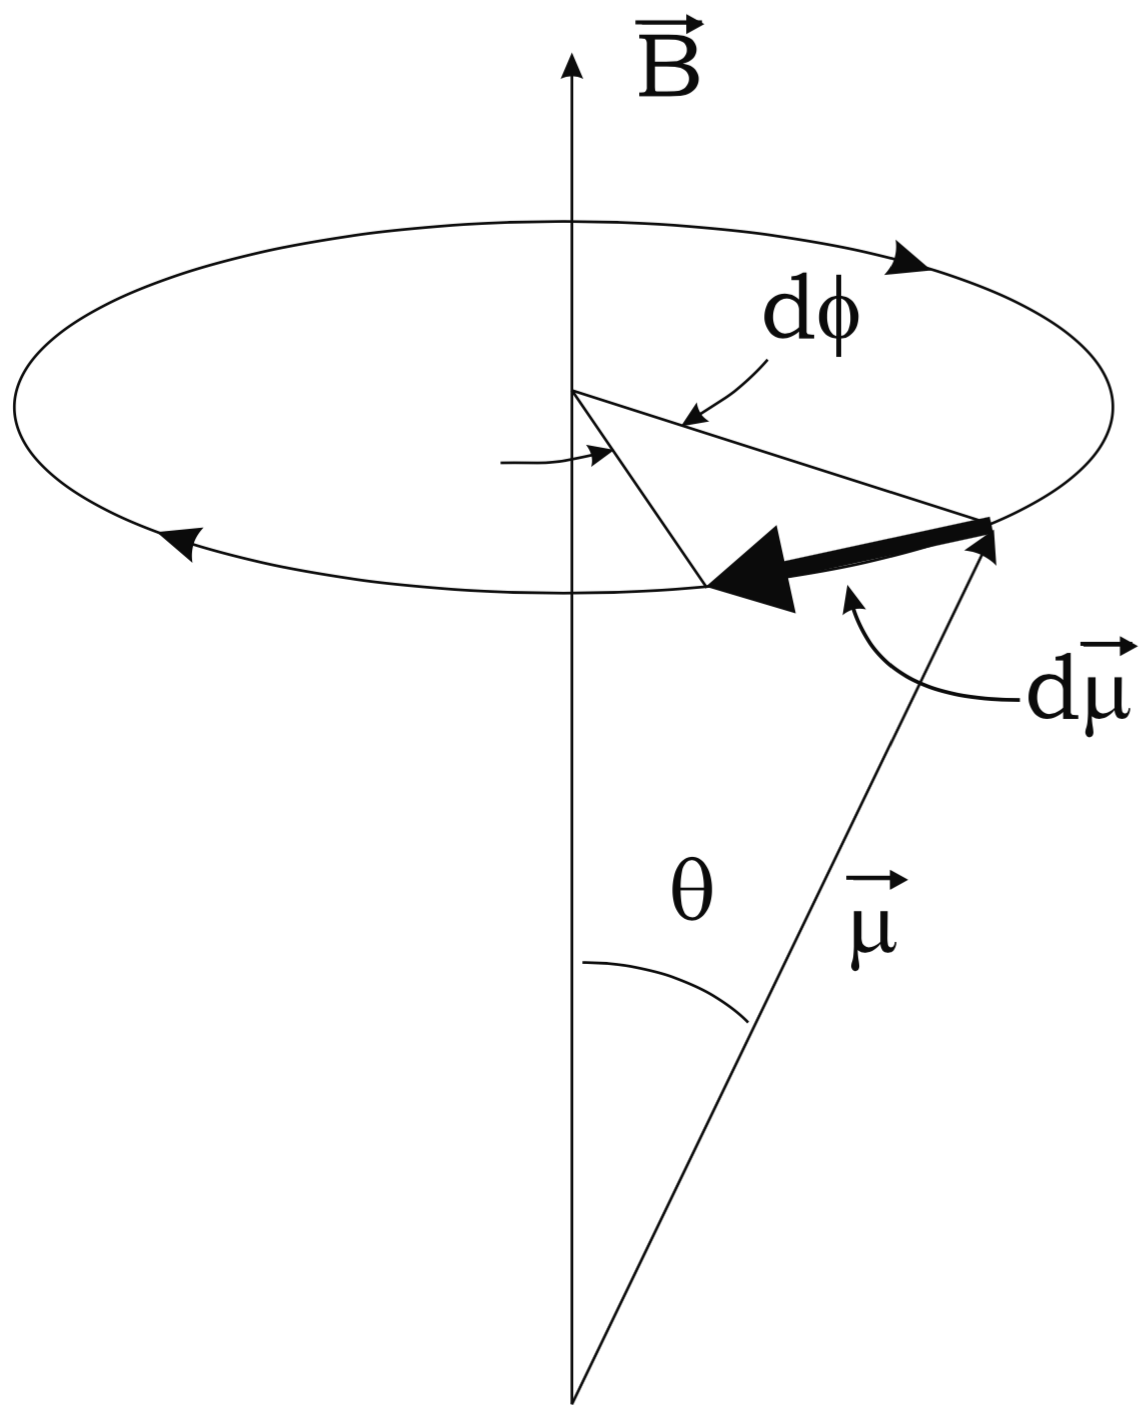
\includegraphics[width=0.4\textwidth,keepaspectratio]{images/mri/ch2precession}
    \caption{Clockwise precession of a proton's spin about a magnetic field. Figure adapted from \cite{Haacke1999}.}
    \label{fig:ch2precession}
\end{figure}

\hfill

% % 4
\textbf{Larmor frequency.} The angular frequency that the magnetic moment $\vec{\mu}$ precesses about the magnetic field in a clockwise fashion is called the \textit{Larmor frequency}:
\begin{equation} \label{eq:28}
	\omega \equiv \Bigl\vert \frac{d \phi}{dt} \Bigr\vert = \gamma \lvert \vec{B} \rvert
\end{equation}

\hfill

% % 5
\textbf{Cartesian representation.}
Considering a static magnetic field $\vec{B} = B_0 \hat{z}$, and a magnetic 
moment pointing in an arbitrary direction, the equation of motion
can be rewritten as follows:
\begin{flalign*}
    \frac{d}{dt}(\mu_x \hat{x} + \mu_y \hat{y} + \mu_z \hat{z}) & = \gamma\, B_0\, (\mu_x \hat{x} + \mu_y \hat{y} + \mu_z\hat{z}) \times \hat{z}\\
    & = \gamma\, B_0\, ( \mu_y \hat{x}  - \mu_x \hat{y} )
\end{flalign*}
The vector differential equation \ref{eq:26} will therefore decompose into 
the three Cartesian equations:
\begin{flalign*}
    \frac{d\mu_x}{dt} & = \phantom{+} \gamma \mu_y B_0 = \phantom{+} \omega_0\,\mu_y \\
    \frac{d\mu_y}{dt} & = - \gamma \mu_x B_0 = - \omega_0\,\mu_x \\
    \frac{d\mu_z}{dt} & = \phantom{+} 0
\end{flalign*}
whose solutions are:
\begin{flalign*}
    {\mu_x}(t) &= {\mu_x}(0) \, cos (\gamma B_0 t) + {\mu_y}(0) \, sin (\gamma B_0 t) \\
    {\mu_y}(t) &= {\mu_y}(0) \, cos (\gamma B_0 t) - {\mu_x}(0) \, sin (\gamma B_0 t) \\
    {\mu_z}(t) &= {\mu_z}(0)
\end{flalign*}

\hfill

% % 6
\textbf{Matrix representation.} A more concise representation of the equation 
of motion of a single spin in a static magnetic field is using matrix notation: 
\begin{equation} \label{eq:27}
	\vec{\mu}(t) = R_z(- \gamma B_0 t) \vec{\mu}(0)
\end{equation}
where 
\begin{flalign*}
	\vec{\mu}(t) & =
    \begin{pmatrix}
	\mu_x(t)\\
	\mu_y(t)\\
	\mu_z(t)
	\end{pmatrix} \text{ and } \omega_0 = -\gamma B_0
\end{flalign*}
and $R_z(\alpha)$ is the matrix representing the anti-clockwise rotation of vectors through an angle $\alpha$:
\begin{flalign*}
	R_z(\alpha) & =
    \begin{pmatrix}
	cos\alpha & -sin\alpha & 0 \\
	sin\alpha & \phantom{+}cos\alpha & 0 \\
	0 & 0 & 1
	\end{pmatrix}
\end{flalign*}
For completion, the rotations about the x and y axis are also presented here:
\begin{flalign*}
	R_x(\alpha) & =
    \begin{pmatrix}
	1 & 0 & 0 \\
	0 & cos\alpha & -sin\alpha \\
	0 & sin\alpha & \phantom{+}cos\alpha 
	\end{pmatrix}
\end{flalign*}
and
\begin{flalign*}
	R_y(\alpha) & =
    \begin{pmatrix}
    \phantom{+}cos\alpha & 0 & sin\alpha \\
	0 & 1 & 0 \\
	-sin\alpha & 0 & cos\alpha  
	\end{pmatrix}
\end{flalign*}

\hfill

% % 7
\textbf{Complex Representation.} Another useful representation of the magnetic moment vector is as a complex number:
\begin{equation} \label{eq:239}
	\mu_+ (t) = \mu_x(t) + i \mu_y(t)
\end{equation}
which allows a very concise representation of the equation of motion:
\begin{equation} \label{eq:240}
	\frac{d\mu_+}{dt} = - i \omega_0 \mu_+
\end{equation}
whose solution is:
\begin{equation} \label{eq:241}
	\mu_+(t) = \mu_+(0) e^{-i \omega_0 t}
\end{equation}

Similarly, by introducing phase into the equation we get:
\begin{equation} \label{eq:244}
	\mu_+(t) = \lvert \mu_+(0) \rvert e^{i \phi_0(t)}
\end{equation}
where the phase is:
\begin{equation} \label{eq:245}
	\phi_0(t) = -\omega_0 t + \phi_0(0)
\end{equation}

\hfill

% % 8
\textbf{Magnetisation.} The magnetic moment vectors of a population of spins 
(also known as an \textit{isochromat}) contained in a volume $V$ give rise to 
a net magnetisation. This vector quantity is called the 
\textit{magnetisation vector} and it is defined as:
\begin{equation} \label{eq:219}
    \vec{M} = \frac{1}{V} \sum_{i \in \text{protons in V}} \vec{\mu}_i
\end{equation}

The equation of motion for the magnetisation vector is the same as for a single spin:
\begin{equation} \label{eq:43}
    \frac{d\vec{M}}{dt} = \gamma \vec{M} \times \vec{B}  \text{  (for non-interacting protons)}
\end{equation}

At thermal equilibrium and when immersed in a constant, static magnetic field 
$\vec{B} = B_0 \, \hat{z}$, the magnetisation vector becomes $\vec{M} = M_0 \, \hat{z}$,
where $M_0$ is found from quantum statistics to be:

\begin{equation} \label{eq:225}
    M_0 = \frac{\gamma^2 \text{\sout{$h$}}^2 \, B_0 \, \rho}{4 \, K \, T}
\end{equation}

In equation \ref{eq:225} we introduced the following quantities: \sout{$h$} $= h/2\pi$ is the reduced Planck constant $h$ ($h = 6.626 \times 10^{-34} J$), also known as \textit{h-bar}, $\rho$ is the number of spins per unit volume 
(spin density), $K$ is the Boltzmann constant 
($1.38 \times 10^{-23} J \, K^{-1}$) and $T$ is the absolute temperature of the system \cite{Haacke1999}. \\

The magnetisation vector $M_0$ is the measured quantity in an MRI experiment. 
As this vector quantity is several orders of magnitude smaller than $B_0$, measuring it 
can only be done by lowering the overall temperature of the object or by increasing the field strength.
In fact, the only actual controllable parameter is the amplitude of the external magnetic field, or $B_0$, which in MRI scanners can range between 0.2 to 9 Tesla, with 1.5T and 3T scanners being the most popular clinically used ones.

\hfill

% % % % % % % % % % % % 
% % % % % % % % % % % % 
\subsection{Radiofrequency Pulse}\label{background:rfpulse}

As stated before, the measurable quantity in MRI is the net 
magnetisation vector. However, in order to be measured, 
the magnetisation vector must be 'tipped' away from its 
thermal equilibrium alignment.
This can be achieved by applying a secondary magnetic field known as the 
\textit{RF Pulse}.
The resulting combined effect of two perpendicular fields leads to a disturbance of any magnetic moment, initially aligned along the original static field, away from that direction. 

\hfill

% % 8
\textbf{Rotating reference frames.} 
The motion of the magnetisation vector while subject to these fields is best described using a new reference frame.
This reference frame is called the \textit{rotating reference frame} and can be distinguished from the \textit{laboratory frame} (stationary frame) by using primed quantities for both the axis of the frame ($x'$, $y'$, $z'$) and their respective unit vectors ($\hat{x}'$, $\hat{y}'$, $\hat{z}'$). 

\hfill

The rotation motion of this frame can be described by the angular velocity vector $\vec{\Omega}$ whose direction and magnitude are the rotation axis and the angular speed of the rotating frame. The rate of change of the magnetisation vector in time relative to the rotating reference frame can be expressed as:
\begin{equation}\label{eq:4433}
    \frac{d \vec{M} (t)}{dt} = \Bigg( \frac{d \vec{M} (t)}{dt} \Bigg)' + \vec{\Omega} \times \vec{M}(t)
\end{equation}

By using equation \ref{eq:43} together with the above equation we get:
\begin{equation}\label{eq:313}
    \Bigg( \frac{d \vec{M} (t)}{dt} \Bigg)' = \gamma \vec{M} \times \vec{B}_{eff}
\end{equation}
where the effective magnetic field in the rotating frame is:
\begin{equation}\label{eq:314}
    \vec{B}_{eff} = \vec{B} + \frac{\vec{\Omega}}{\gamma}
\end{equation}

This is a key equation in MR as it shows that from the primed reference frame perspective, the magnetisation vector is rotated due to the presence of a total (or effective) magnetic field. The choice of $\vec{\Omega}$ is then equal to $- \gamma \vec{B}$ such that the magnetisation vector will lie still in the rotating reference frame.

\hfill

% % 9
\textbf{RF Field.} By introducing a new magnetic field which is perpendicular to the main magnetic field, the magnetisation vector can be 'tipped' away from the $\hat{z}$ axis. This field is called the \textit{transmit RF field} ($\vec{B_1}$) and it is most effective when it is a \textit{left-circularly polarized} magnetic field. Specifically, the RF field used in MRI is:
\begin{equation}\label{eq:324}
    \vec{B}_{1}^{cir} = B_1 (\hat{x} \, cos \, \omega t - \hat{y} \, sin \, \omega t)
\end{equation}
which makes it static in the rotating reference frame:
\begin{equation}\label{eq:325}
    \vec{B}_{1}^{cir} = B_1 \hat{x}'
\end{equation}

When combining the constant magnetic field $\vec{B_0} = B_0 \hat{z}$ with the left-circularly polarised field $\vec{B_1} = B_1 \hat{x}'$ and setting $\hat{z}' = \hat{z}$ we get:
\begin{equation}\label{eq:326}
    \Bigg( \frac{d \vec{M} }{dt} \Bigg)' = \vec{M} \times [ \hat{z}'  (\omega_0 - \omega) + \hat{x}' \omega_1]
\end{equation}
where $\omega_0 \equiv \gamma B_0$ is the Larmor frequency, $\omega$ is the rf laboratory frequency and $\omega_1 \equiv \gamma B_1$ is the precession frequency induced by the rf field.

The effective magnetic field will therefore be:
\begin{equation}\label{eq:328}
    \vec{B}_{eff} \equiv [ \hat{z}'  (\omega_0 - \omega) + \hat{x}' \omega_1] / \gamma
\end{equation}

\hfill

% % 10
\textbf{On-resonance Condition.} 
In MRI the applied RF field's frequency $\omega$ is chose such that it matches the Larmor frequency $\omega_0$. 
This is called the \textit{on-resonance condition} and it leads to the cornerstone equation of motion:
\begin{equation}\label{eq:329}
    \Bigg( \frac{d \vec{M}}{dt} \Bigg)' = \omega_1 \vec{M} \times \hat{x}'
\end{equation}
where the $B_1$ field is maximally synchronised to tip the spin about the $\hat{x}'$ axis.

\hfill

% % 11
\textbf{RF Pulse.} \label{app:rfpulse}
An on-resonance RF transmit field applied for a finite time is called an \textit{rf pulse}. 
The magnitude of the $B_1$ field and the amount of time $\tau$ it is turned on can be adjusted to control for the angle of rotation. 
This angle is called \textit{flip angle} and is related to the other two quantities through the following formula:
\begin{equation}\label{eq:331}
    \Delta \theta = \gamma B_1 \tau
\end{equation}
For example, a $\pi/2$ flip can be achieved in $1.0 ms$ with a $B_1$ field of $5.9 \mu T$ for hydrogen protons \cite{Haacke1999}. 
The trajectory of the magnetisation vector undergoing this motion is illustrated in Figure~\ref{fig:ch3spintrajboth}.

\begin{figure}[ht]
    \centering
    \begin{subfigure}[b]{0.45\textwidth}
        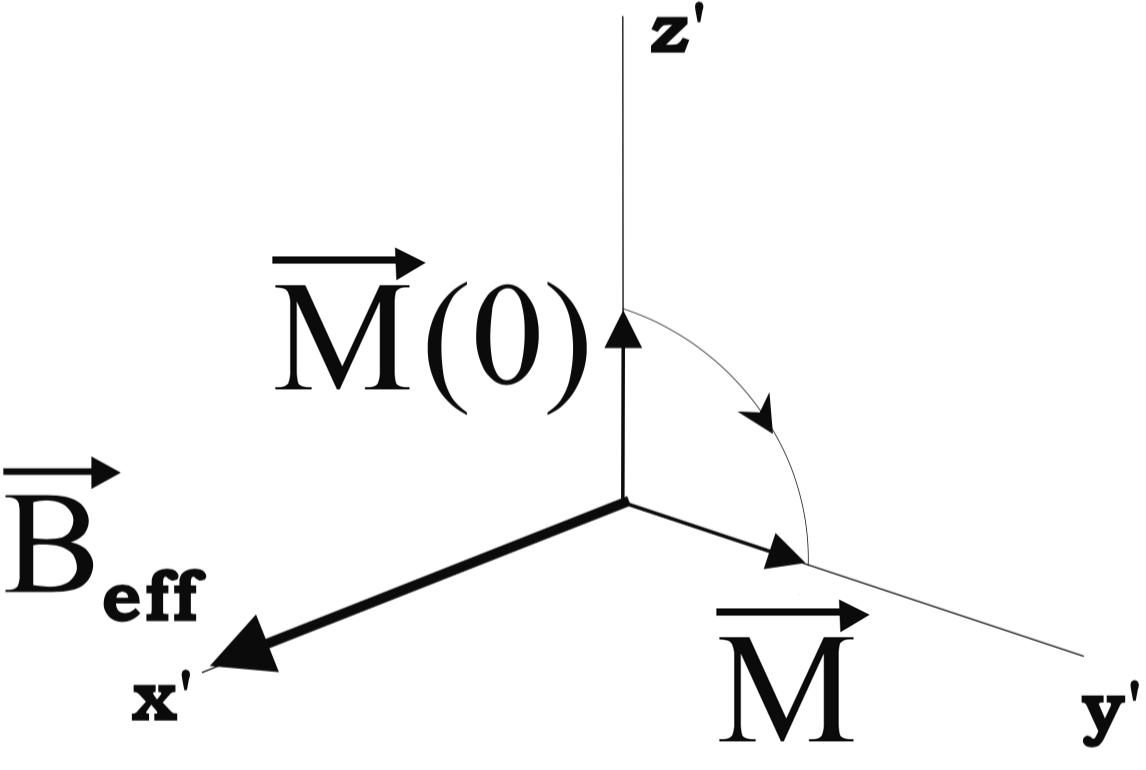
\includegraphics[width=\textwidth]{images/mri/ch3spintraja}
        \caption{Rotating frame}
        \label{fig:ch3spintraja}
    \end{subfigure}
    ~ %add desired spacing between images, e. g. ~, \quad, \qquad, \hfill etc. 
      %(or a blank line to force the subfigure onto a new line)
    \begin{subfigure}[b]{0.4\textwidth}
        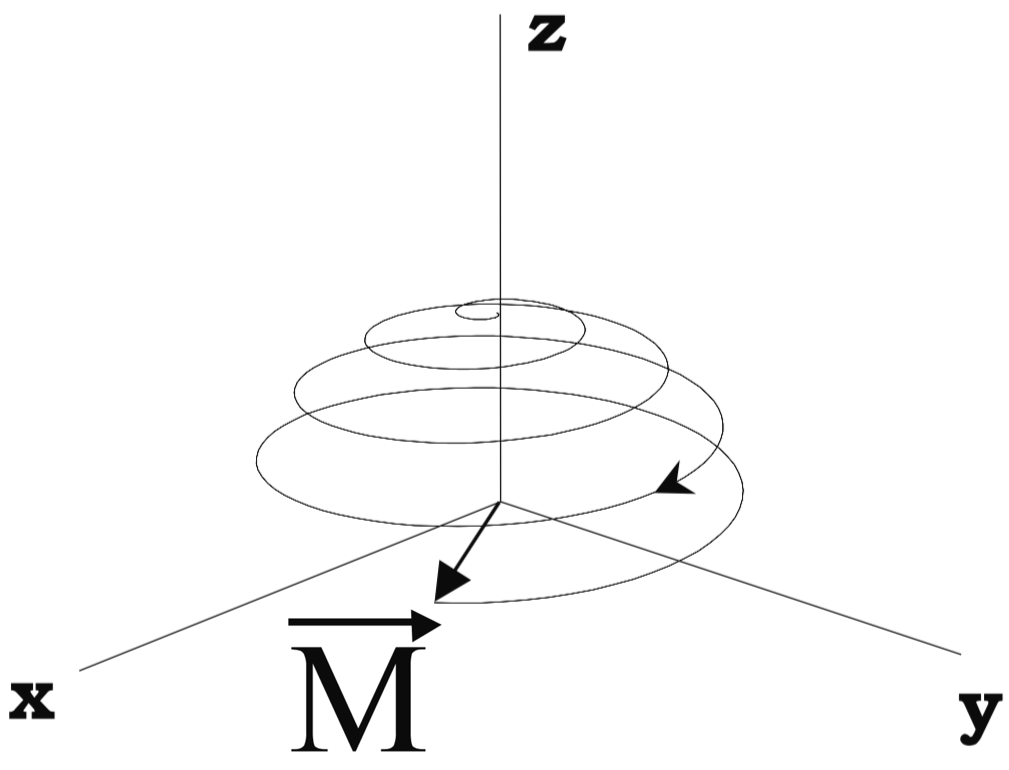
\includegraphics[width=\textwidth]{images/mri/ch3spintrajb}
        \caption{Laboratory frame}
        \label{fig:ch3spintrajb}
    \end{subfigure}
    
    \caption{Magnetisation vector trajectory in both the rotating and the laboratory frame. Figure adapted from \cite{Haacke1999}}
    \label{fig:ch3spintrajboth}
\end{figure}

\hfill

In most MR experiments, the RF pulse has a very short duration (a few milliseconds).
It can therefore be assumed that it happens instantaneously and that there are no relaxation effects during its application.
Mathematically, an instantaneous RF pulse of flip angle $\alpha$ and initial phase $\phi$ can be described with rotation matrices.
The post-RF pulse magnetisation vector $\vec{M}$ will therefore depend on its pre-RF pulse state $\vec{M}(0)$ by the following equation
\begin{equation} \label{eq:445}
    M = R_z(\phi) R_x(-\alpha) R_z(-\phi) M(0)
\end{equation}

For a perfect $\pi/2$ pulse applied uniformly over the sample, the post-RF magnetisation vector will be the equilibrium magnetisation $M_0$. 
From equation ~\ref{eq:225} we can now write:
\begin{equation}\label{eq:93}
    M_{\perp}(\vec{r},0) = M_0(\vec{r}) = \rho_0(\vec{r}) \frac{\gamma^2 \text{\sout{$h$}}^2 \, B_0}{4 \, K \, T}
\end{equation}
which introduces the spin density $\rho_0$.

\hfill

% % % % % % % % % % % % 
% % % % % % % % % % % % 
\subsection{Relaxation} \label{app:relaxation}

The picture we have painted so far refers to non-interacting spins.
As expressed in equation \ref{eq:43}, the equation of motion for the magnetisation vector is $\frac{d\vec{M}}{dt} = \gamma \vec{M} \times \vec{B}$  for non-interacting protons. 
This equation can be decomposed into its parallel ($\vec{M}_{||} = M_z \hat{z}$) and longitudinal ($\vec{M}_{\perp} = M_X \hat{x} + M_y \hat{y}$) components which yield the following decoupled equations:
\begin{equation}\label{eq:46}
    \frac{d M_z}{dt} = 0
\end{equation}
and 
\begin{equation}\label{eq:47}
    \frac{d \vec{M}_{\perp}}{dt} = \gamma \vec{M}_{\perp} \times \vec{B}_{ext}
\end{equation}
for non-interacting protons.

\hfill

% % 12
\textbf{Interacting protons.} In reality, the hydrogen protons contained in a sample are constantly interacting with their environment and with each other.
The result of this interaction leads to additional terms in the equations above.
These terms will depend on some decay parameters which are different for both of these equations.
This means that the magnetisation vector components will 'relax' differently to their equilibrium values.

\hfill

% % 13
\textbf{Spin-Lattice Relaxation.} The relaxation of the longitudinal component to its thermal equilibrium is called the \textit{spin-lattice relaxation}. 
When the magnetisation is disturbed by an external magnetic field such as an RF pulse, the spin system gains potential energy.
By releasing this energy back to the lattice, the magnetisation then returns to its equilibrium.
This process takes the form of an exponential recovery and it is described by the following empirical relation:
\begin{equation}\label{eq:411}
    \frac{d \vec{M}_{z}}{dt} = \frac{1}{T_1} (M_0 - M_z) \hat{z}
\end{equation}
where $T_1$ is known as the \textit{spin-lattice relaxation time} and its solution is:
\begin{equation}\label{eq:413}
    M_z(t) = M_z(0) e^{-t/T_1} + M_0(1-e^{-t/T_1}) \, \text{ (for } \vec{B}_0 \parallel \hat{z} \text{)}
\end{equation}

\hfill

% % 14
\textbf{Spin-Spin Relaxation.} The relaxation of the transverse component to its thermal equilibrium is called the \textit{spin-spin relaxation}. 
This phenomena happens due to the interaction between individual spins.
These interactions cause local magnetic field changes which lead to variations in the precessional frequencies of the spins.
As a consequence, the magnetic moment vectors will gain or lose phase with respect to the expected Larmor frequency.
Over time, this process will cause a complete dephasing of the system which will, in turn, lead to a zero net magnetisation vector.
To characterize this phenomena we use the $T_2$ \textit{spin-spin relaxation time} and the following empirical relation:
\begin{equation}\label{eq:412}
    \frac{d \vec{M}_{\perp}}{dt} = \gamma \vec{M} \times \vec{B} - \frac{1}{T_2} \vec{M}_{\perp}
\end{equation}
with solution:
\begin{equation}\label{eq:414}
    \vec{M}_{\perp}(t) = \vec{M}_{\perp}(0) e^{-t/T_2} \, \text{ (in the rotating frame)}
\end{equation}

\hfill

% % 15
\textbf{The $\mathbf{T_2^*}$ relaxation term.} 
In reality, the transverse relaxation rate is higher than described above because of external field inhomogeneities.
This process is characterised by a separate decay rate called $R_2' \equiv 1/T_2'$ and together with the intrinsic decay rate $R_2 \equiv 1/T_2$ yields the total relaxation rate $R_2^* = R_2 + R_2'$.
By inverting this equation we arrive with:
\begin{equation} \label{eq:420}
    \frac{1}{T_2^*} = \frac{1}{T_2} + \frac{1}{T_2'}
\end{equation}
where ${T_2^*} \equiv 1/R_2^*$.
It is worth mentioning that the loss in transverse magnetisation due to external field inhomogeneities $T_2'$ is 'recoverable' in MRI, while the intrinsic $T_2$ losses are not.

\hfill

% % % % % % % % % % % % 
% % % % % % % % % % % % 
\subsection{Off-resonance Effects}

Inhomogeneities in the main magnetic field directly affect the spins' precession frequencies.
As stated before, the frequency of precession for a given spin is proportional to the gyromagnetic ratio and the magnitude of the magnetic field (equation \ref{eq:28}).
Any deviation from the expected $B_0$ value will therefore change the precession frequency to:
\begin{equation}\label{eq:omegaEffects}
    \omega = \gamma \lvert \vec{B}_0 + \Delta \vec{B} \rvert = \omega_0 + \Delta \omega
\end{equation}
where $\Delta \omega$ is the off-resonance frequency.

\hfill

% % % % % % % % % % % % 
% % % % % % % % % % % % 
\subsection{Bloch Equation}
\label{chapterlabel2sec1Bloch}

The combined effect of both spin-lattice and spin-spin relaxations in one equation is called \textit{the Bloch equation}. 
This equation takes the following form:

\begin{equation} \label{eq:421}
    \frac{d\vec{M}}{dt} = \gamma \vec{M} \times \vec{B} + \frac{1}{T_1} (M_0 - M_z) \hat{z} - \frac{1}{T_2} \vec{M}_{\perp}
\end{equation} 

which can be decomposed in its $x/y/z$ components:
\begin{equation} \label{eq:422}
    \frac{dM_z}{dt} = \frac{M_0 - M_z}{T_1}
\end{equation}
\begin{equation} \label{eq:423}
    \frac{dM_x}{dt} = \omega_0 M_y - \frac{M_x}{T_2}
\end{equation}
\begin{equation} \label{eq:424}
    \frac{dM_x}{dt} = -\omega_0 M_x - \frac{M_y}{T_2}
\end{equation}
for $\vec{B} = B_0 \hat{z}$ and $\omega_0 = \gamma B_0$.

\hfill

% % 15
\textbf{Solutions to the Bloch equation.} 
The solutions for the equations above are:
\begin{equation} \label{eq:425}
    M_x(t) = e^{-t/T_2} (M_x(0) \, cos \, \omega_0 t + M_y(0) \, sin \, \omega_0 t)
\end{equation}
\begin{equation} \label{eq:426}
    M_y(t) = e^{-t/T_2} (M_y(0) \, cos \, \omega_0 t - M_x(0) \, sin \, \omega_0 t)
\end{equation}
\begin{equation} \label{eq:427}
    M_z(t) = M_z(0) e^{-t/T_1} + M_0 (1 - e^{-t/T_1})
\end{equation}
which reach $M_x(\infty) = M_y(\infty) = 0$ and $M_z(\infty) = M_0$ in the asymptotic limit $t \rightarrow \infty$.

Figure~\ref{fig:ch4MxMyMz} shows the behaviour of the magnetisation vector components in time for a sample with $T_1 = 600 \, ms$ and $T_2 = 80 \, ms$ at $B_0 = 1.5T$, which corresponds to white matter.

\begin{figure}[ht]
    \centering
    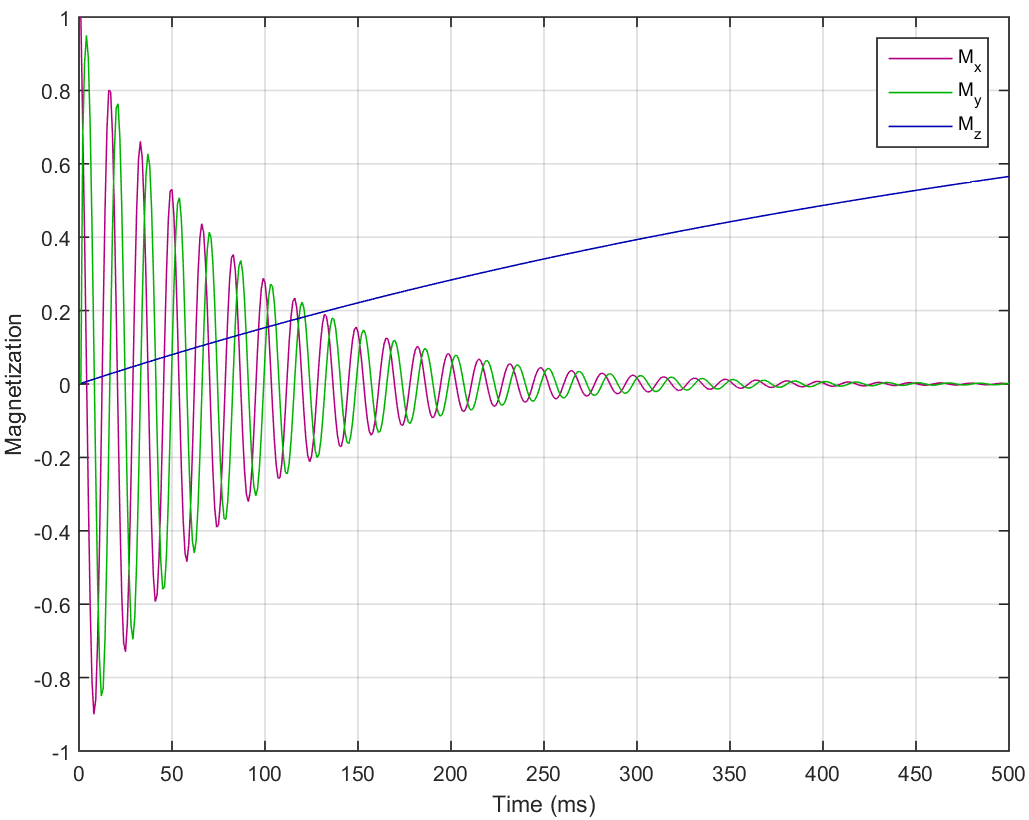
\includegraphics[width=0.9\textwidth,keepaspectratio]{images/mri/ch4MxMyMz}
    \caption{Relaxation in the laboratory frame. This figure shows the regrowth of the longitudinal component of the magnetization vector from 0 to its initial value $M_0$ in blue and the decay of both transverse components from an initial value to 0 in purple and green. $M_0$ is considered to be equal to 1 for illustration purposes.}
    \label{fig:ch4MxMyMz}
\end{figure}

\hfill

% % 16
\textbf{Matrix representation.}\label{app:matrixbloch} A useful representation for the Bloch equation is the \textit{matrix representation}.
By constructing a diagonal matrix $D$ with the $T_1$ and $T_2$ decay factors:
\begin{equation}
    D ( t ) = \left[
    \begin{array}{c c c}
          e^{-t/T_2} &     0      &     0 \\
              0      & e^{-t/T_2} &     0 \\
              0      &     0      & e^{-t/T_1}
    \end{array}
    \right]
\end{equation}
a column matrix $C$:
\begin{equation}
    C ( t ) = \left[
    \begin{array}{c}
        0 \\
        0 \\
    M_0(1 - e^{-t/T_1})
    \end{array}
    \right]
\end{equation}
and the previously defined rotation matrix $R_z$ we get:

\begin{equation} \label{eq:444}
    M(t) = D(t) R_z(-\omega_0 t) M(0) + C(t)
\end{equation}
where $M(t)$ is:
\begin{equation}
    M ( t ) = \left[
    \begin{array}{c}
        M_x(t) \\
        M_y(t) \\
        M_z(t)
    \end{array}
    \right]
\end{equation}
and $M(0)$ is the magnetisation vector immediately after it has been flipped by an instantaneous RF pulse.

% % % % % % % % % % % % % % % % 
\section{Image Formation}\label{chapterlabel2sec12}
After establishing the mathematical framework for how protons react to being subjected to a variety of magnetic fields we are now in the position of discussing how images are formed in MRI.
This section focuses on describing how MR images are obtained, from signal acquisition to image reconstruction. 

\hfill

% % % % % % % % % % % % 
% % % % % % % % % % % % 
\subsection{Signal Detection}

An important step towards image formation is the signal acquisition process. 
The precession motion of the magnetisation vector in the transverse plane can be detected by measuring the induced voltage in a receiver coil. 
The law that governs this phenomena is called the \textit{Faraday's lay of electromagnetic induction}.
It states that the induced voltage (\textit{emf}) is proportional to the rate of change of the magnetic flux ($\Phi$) through the coil:
\begin{equation} \label{eq:71}
    emf = - \frac{d \Phi(t)}{dt}
\end{equation}
where 
\begin{equation}\label{eq:72}
    \Phi(t) = \int_{sample} \vec{B}^{receive}(\vec{r}) \cdot \vec{M}(\vec{r}, t) d\vec{r}
\end{equation}
and $\vec{B}^{receive}(\vec{r})$ is the detection coil's 'received' magnetic field at position $\vec{r}$, and $\vec{M}(\vec{r}, t)$ is the magnetization vector at position $\vec{r}$ and time $t$.
A full derivation of equation \ref{eq:72} can be found in \cite{Haacke1999}. 
The signal through time $S(t)$ is proportional to the electromotive force:
\begin{equation}\label{eq:714}
    S(t) \propto V(t) = - \frac{d }{d t} \int_{sample} \vec{B}^{receive}(\vec{r}) \cdot \vec{M}(\vec{r}, t) d\vec{r}
\end{equation}
which in its decomposed form looks like:
\begin{equation}
    S(t) \propto - \frac{d}{dt} 
    \int_{sample}
          [B_x^{receive} (\vec{r}) M_x (\vec{r}, t) + 
          B_y^{receive} (\vec{r}) M_y (\vec{r}, t) + 
          B_z^{receive} (\vec{r}) M_z (\vec{r}, t)]  d\vec{r}
\end{equation}

After further simplifications and derivations, the details of which can be found in \cite{Haacke1999}, the signal expression known in MRI becomes:
\begin{equation}
    S(t) =
        \omega_0 \int_{sample} e^{-t/T_2(\vec{r})} M_{\perp}(\vec{r},0) 
            B_{\perp}(\vec{r}) sin(\omega_0 t + \theta_B(\vec{r}) - \phi_0(\vec{r})) d\vec{r}
\end{equation}
where $\phi_0$ is the initial phase of $\vec{M}_{\perp}$ after the RF pulse 
and $\theta_B$ is the receive field angle.
The equation can be modified to incorporate external field inhomogeneities by replacing $T_2$ with $T_2^*$.

\hfill

% % 17
\textbf{Signal demodulation.} In order to view the signal from the perspective of a rotating reference frame, the rapid $\omega_0$ oscillations are removed through a process called \textit{demodulation}.
In short, the signal is multiplied with a (co)sinusoid with a frequency that matches the $\omega_0$ Larmor frequency as close as possible.
The result of this process results in both a 'real' and an 'imaginary' channel for the signal.

By representing the magnetisation vector in its complex form:
\begin{equation}\label{eq:716}
\begin{aligned}
    M_{+}(\vec{r},t) \equiv M_x(\vec{r},t) + i M_y(\vec{r},t) &= e^{- t/T_2(\vec{r})} e^{-i \omega_0 t } M_+(\vec{r},0) \\
    &= e^{- t/T_2(\vec{r})} e^{-i \omega_0 t + i \phi_0(\vec{r})} M_{\perp}(\vec{r},0)
\end{aligned}
\end{equation}
as well as the receive field:
\begin{equation}\label{eq:729}
    B_{+} \equiv B_x^{receive} + i B_y^{receive} = B_{\perp} e^{i \theta_B}
\end{equation}
the compound complex signal becomes:
\begin{equation}\label{eq:730}
    s(t) \equiv s_{re}(t) + i s_{im}(t) \propto \omega_0 \int d^3 r \, \,  M_{+}(\vec{r},t) B^*_{+}(\vec{r})
\end{equation}

\hfill

% % % % % % % % % % % % 
% % % % % % % % % % % % 
\subsection{Spatial Encoding and K-Space Representation}

The signal we described so far is the global signal arising from the entire sample.
However, the goal of MRI is to determine the spatial distribution of the spins.
This can be achieved through spatially varying the magnetic field in such a way that different spins will precess at different rates based on their locations.

\hfill 

% % % % 
\textbf{Imaging Gradients} These variations in the main magnetic field can be achieved through \textit{gradient fields} which are defined by:
\begin{equation}
    \begin{split}
        \vec{G}(t) & \equiv \nabla B_{G_z}(\vec{r}, t) \\
                  &    =   \frac{\partial B_{G_z}(\vec{r},t)}{\partial x} \hat{x} + \frac{\partial B_{G_z}(\vec{r},t)}{\partial y} \hat{y} + \frac{\partial B_{G_z}(\vec{r},t)}{\partial z} \hat{z} \\
                  & \equiv G_x(t) \hat{x} + G_y(t) \hat{y} + G_z(t) \hat{z}
    \end{split}
\end{equation}
where $\vec{r}$ is a displacement vector from the isocenter and 
$G_x$, $G_y$ and $G_z$ are the components of the gradient field $\vec{G}$.
When a gradient field is superimposed over the main magnetic field, 
the total magnetic field at any location $\vec{r}$ is given by:
\begin{equation}
    \vec{B}(\vec{r},t) = (B_0 + \vec{G}(t) \cdot \vec{r}) \hat{z} = (B_0 + B_{G_z}(\vec{r}, t))\hat{z} = (B_0 + G_x(t)x + G_y(t)y + G_z(t)z) \hat{z}
\end{equation}

This equation can be rewritten in terms of the angular frequency of the precessing spins:
\begin{equation} \label{eq:910}
    \omega(\vec{r}, t) = \gamma \lvert \vec{B}(\vec{r}, t) \rvert = \gamma B_0 + \gamma B_{G_z} (\vec{r}, t) = \omega_0 + \gamma \vec{G}(t) \cdot \vec{r}
\end{equation}
which makes the connection between spatial coordinates and frequency of precession.

\hfill

% % % % 
\textbf{Spatial Selectivity}
In order to excite a certain part of the sample (slice selection), an RF pulse is applied together with a magnetic field gradient.
The angular frequency of the spins at location $z$ is given by the following equation:
\begin{equation} \label{eq:911}
    \omega(z) = \gamma B_0 + \gamma \vec{G} \cdot \vec{r} = \omega_0 + \gamma G_z z
\end{equation}
which, in frequency terms, becomes:
\begin{equation} \label{eq:912}
    \nu(z) = \nu_0 + \text{\sout{$\gamma$} } G_z z
\end{equation}
where $\nu_0$ is the frequency of the spins at the isocenter.

\hfill

The slice selection process can be modified to excite any slice at position $\delta z$ from the isocenter by changing the carrier frequency of the RF pulse with the offset $\delta \nu_{RF}$:
\begin{equation} \label{eq:913}
    \delta \nu_{RF} = \text{\sout{$\gamma$} } G_z \delta z
\end{equation}
The thickness of the slice is controlled by the RF pulse's transmit bandwidth of frequencies $\Delta \nu_{RF}$:
\begin{equation} \label{eq:914}
    \Delta z = \frac{\Delta \nu_{RF}}{\text{\sout{$\gamma$} } G_z} 
\end{equation}

The relationship between these terms can be seen in Figure~\ref{fig:ch9sliceselect}.

\begin{figure}[ht]
    \centering
    \begin{subfigure}[b]{0.48\textwidth}
        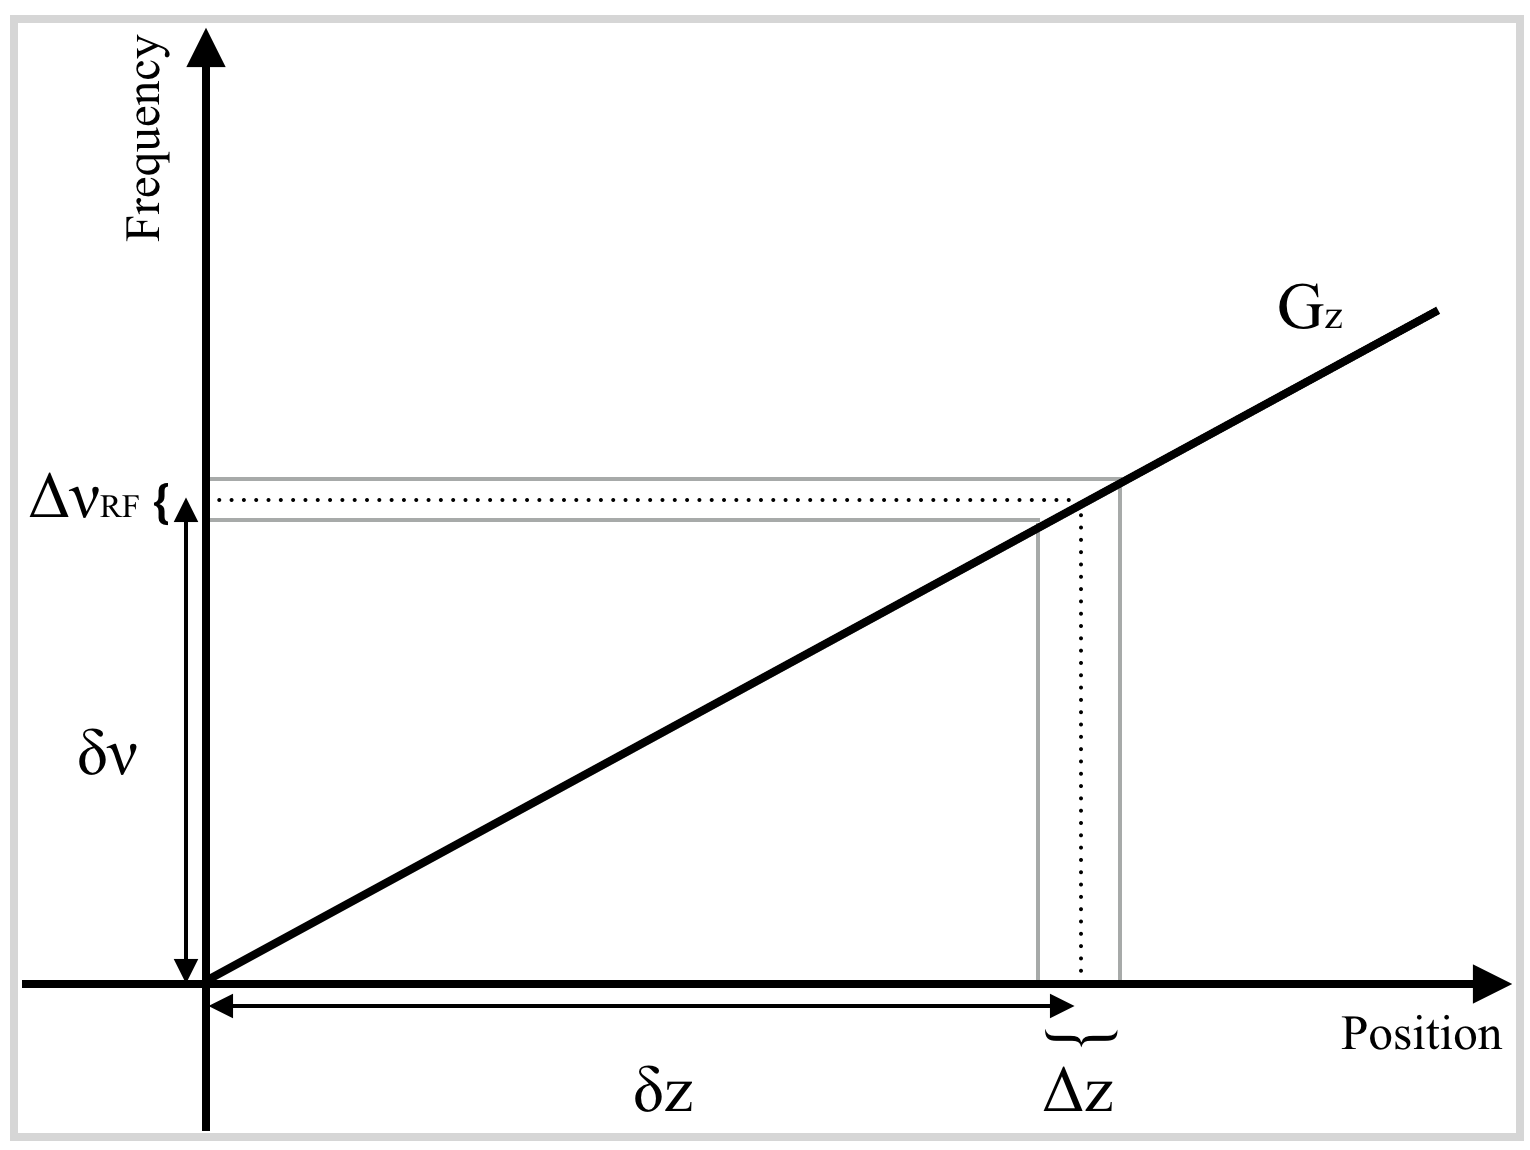
\includegraphics[width=\textwidth]{images/mri/ch9sliceselect1}
        \caption{Selection of slice at position $\delta z$ from the isocentre.}
        \label{fig:ch9sliceselect1}
    \end{subfigure}
    ~ %add desired spacing between images, e. g. ~, \quad, \qquad, \hfill etc. 
      %(or a blank line to force the subfigure onto a new line)
    \begin{subfigure}[b]{0.48\textwidth}
        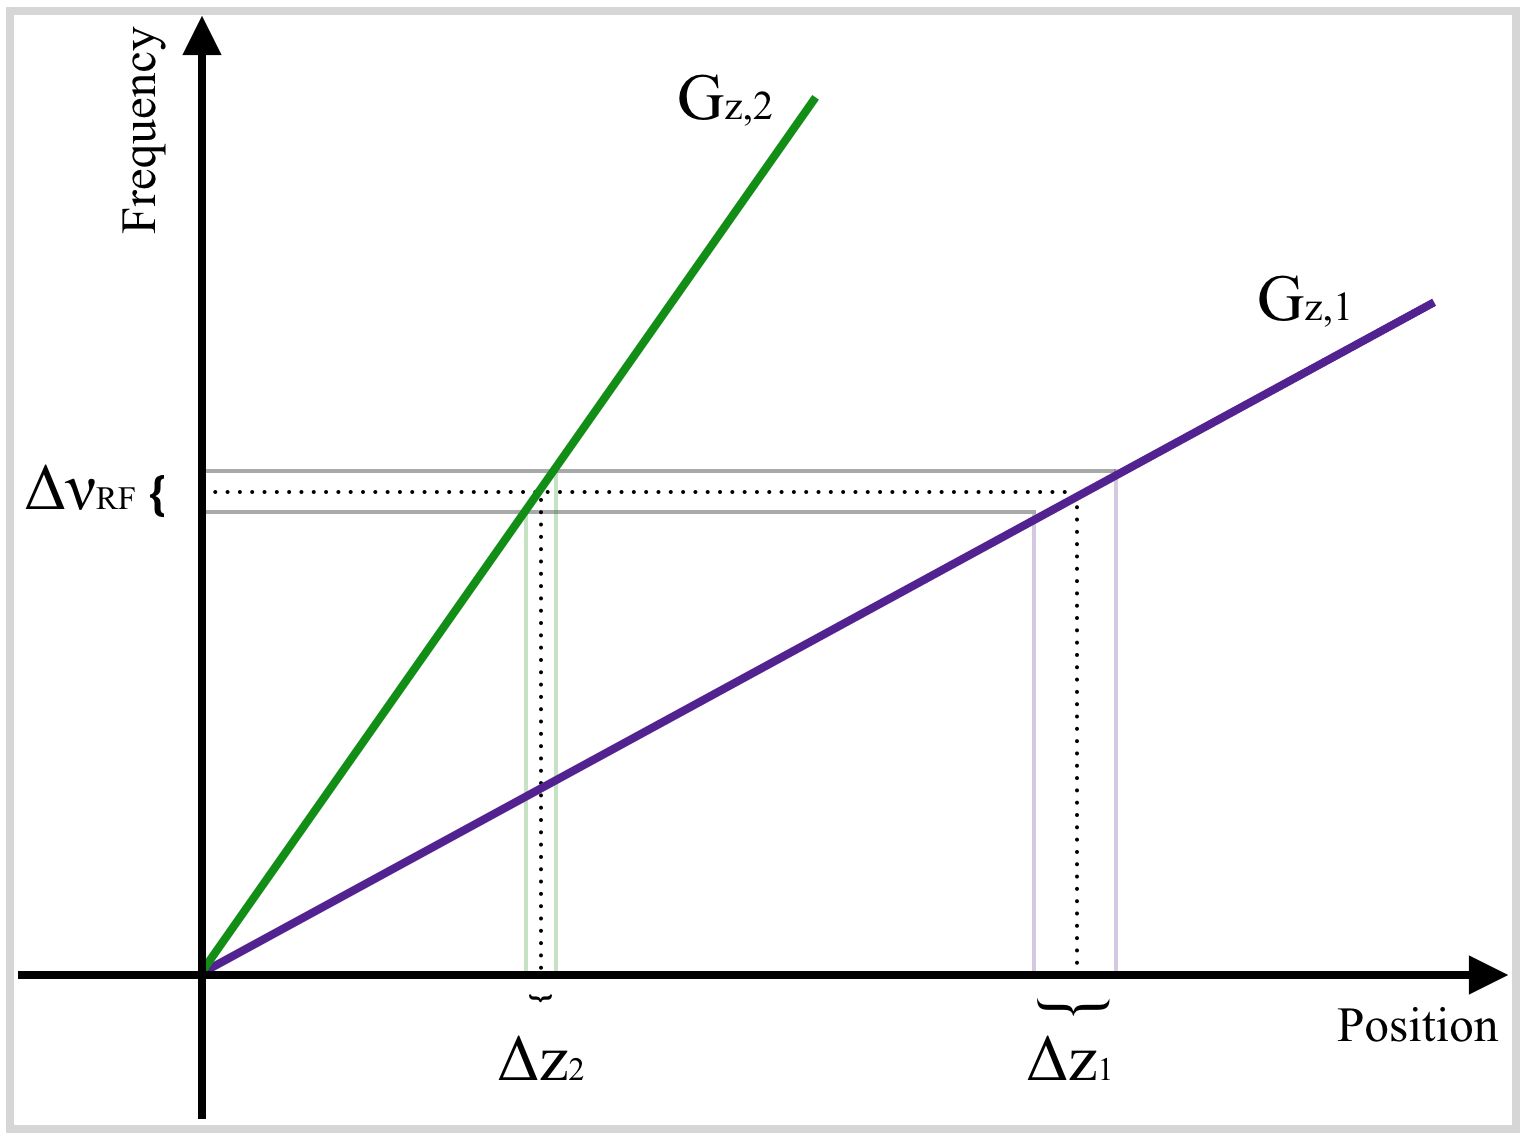
\includegraphics[width=\textwidth]{images/mri/ch9sliceselect2}
        \caption{Selection of slice thickness by controlling the gradient's strength.}
        \label{fig:ch9sliceselect2}
    \end{subfigure}
    
    \caption{The relationship between gradient strength, carrier frequency offset, frequency bandwidth, slice thickness and slice localistion.}
    \label{fig:ch9sliceselect}
\end{figure}

\hfill

% % % % 
\textbf{Frequency Encoding} After the selection of a certain slice, spatial encoding within the plane is performed. 
The first step of that process is called \textit{frequency encoding} and it is achieved by applying a linear gradient in one of the plane's directions.
For example, for a gradient $\vec{G}_{FE}$, the frequency of the spins will be linearly dependent the gradient's direction:
\begin{equation}
    \omega(\vec{r},t) = \omega_0 + \gamma \vec{G}_{FE}(t) \cdot \vec{r}
\end{equation}
A visual illustration of this process happening for a linear gradient in the x direction is shown in Figure~\ref{fig:ch10freqenc}.

\hfill

By taking equation \ref{eq:93} into account, the signal collected while the frequency encoding gradient is on will have the following general form:
\begin{equation}
    s(t) = \int_{sample} \rho(\vec{r}) e^{-t/T_2^*} e^{i \phi_{G_{FE}}(\vec{r}, t)}
\end{equation}
where $\phi_{G_{FE}} = - \gamma \int_{0}^{t} dt' G_{FE}(t') \cdot \vec{r}$ is the accumulated phase due to the application of the gradient and $\rho(\vec{r})$ is the spin density at position $\vec{r}$. 

\hfill

% % % % 
\textbf{Phase Encoding} The second step is called \textit{phase encoding}.
This process is similar to the frequency encoding one, with the exception that the gradient is played for a finite amount of time and then turned off before the signal is acquired. 
The spins will accumulate different phases depending on their spatial location during this time and that phase will be 'remembered' thereafter.
For a phase encoding gradient $G_{PE}$ applied for $\tau_{PE}$ time, the accumulated phase at each location $\vec{r}$ will take the following form:
\begin{equation}
    \phi(\vec{r}) = \gamma \vec{G}_{PE} \cdot \vec{r} \, \, \tau_{PE}
\end{equation}

The total received signal after the gradient was turned off will be:
\begin{equation}
    s(t) = \int_{sample} \rho(\vec{r}) e^{-t/T_2^*} e^{i \phi_{G_{PE}}(\vec{r}, t)}
\end{equation}
where $\phi_{G_{PE}} = - \gamma \int_{0}^{t} dt' G_{PE}(t') \cdot \vec{r}$. 
Figure~\ref{fig:ch10phaseenc} shows a visual illustration of this process happening for a linear gradient in the x direction.

\begin{figure}[ht]
    \centering
    \begin{subfigure}[b]{0.48\textwidth}
        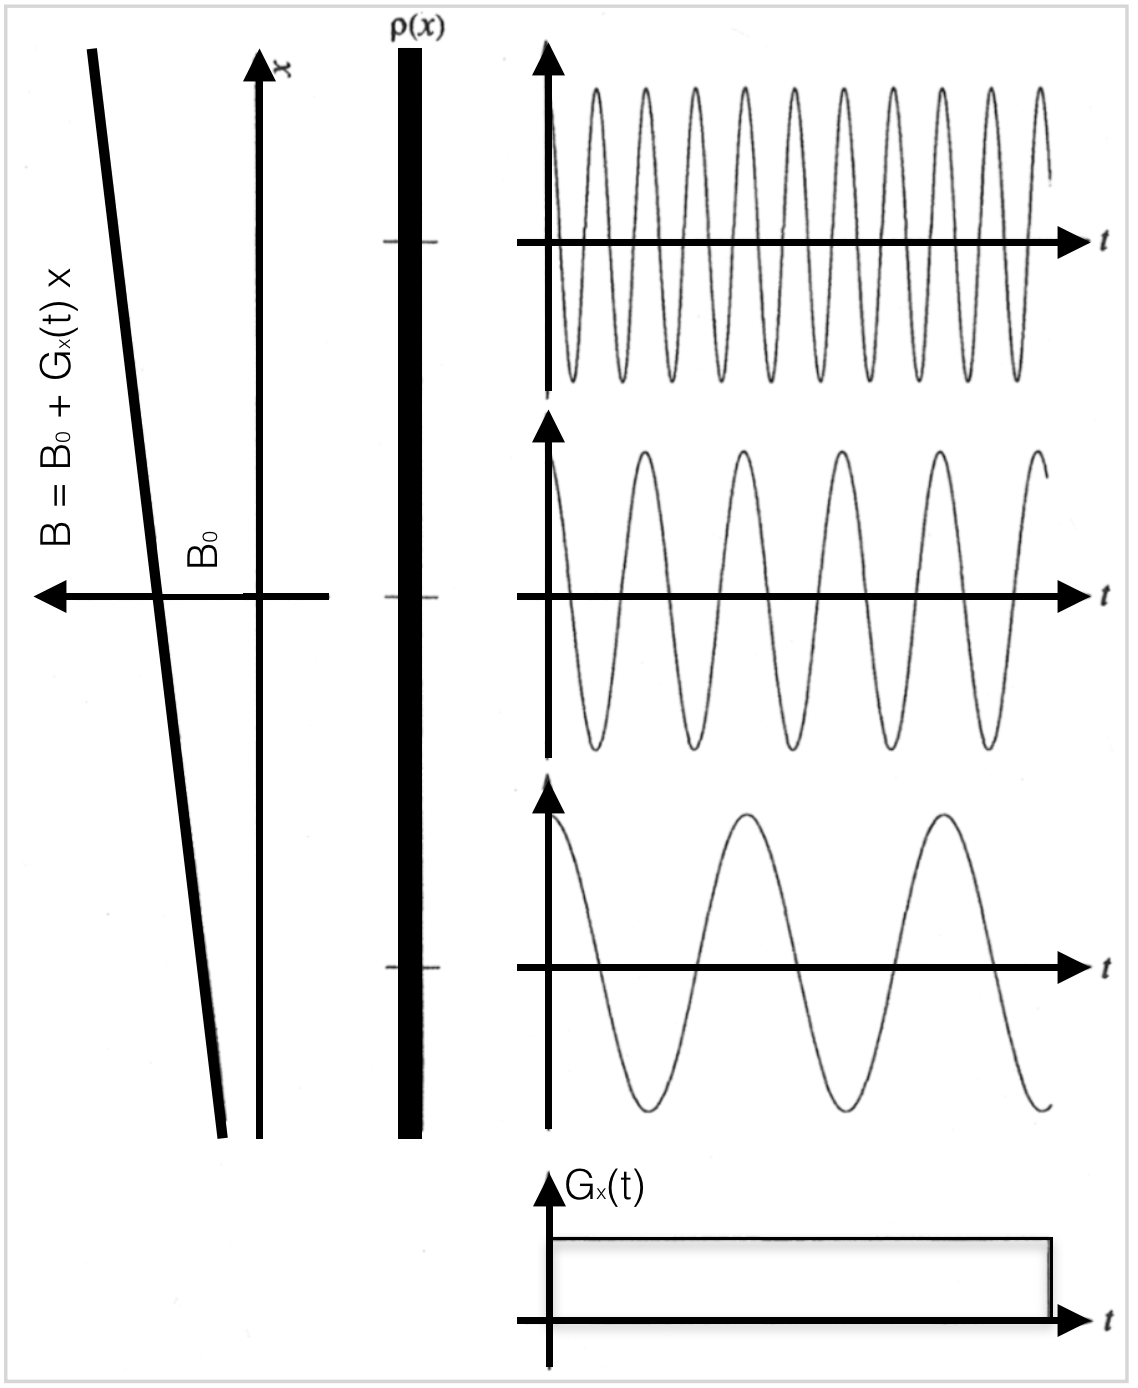
\includegraphics[width=\textwidth]{images/mri/ch10freqenc}
        \caption{Example of how the frequency encoding gradient will affect the signal arising from different locations within a spin system.}
        \label{fig:ch10freqenc}
    \end{subfigure}
    ~ %add desired spacing between images, e. g. ~, \quad, \qquad, \hfill etc. 
      %(or a blank line to force the subfigure onto a new line)
    \begin{subfigure}[b]{0.48\textwidth}
        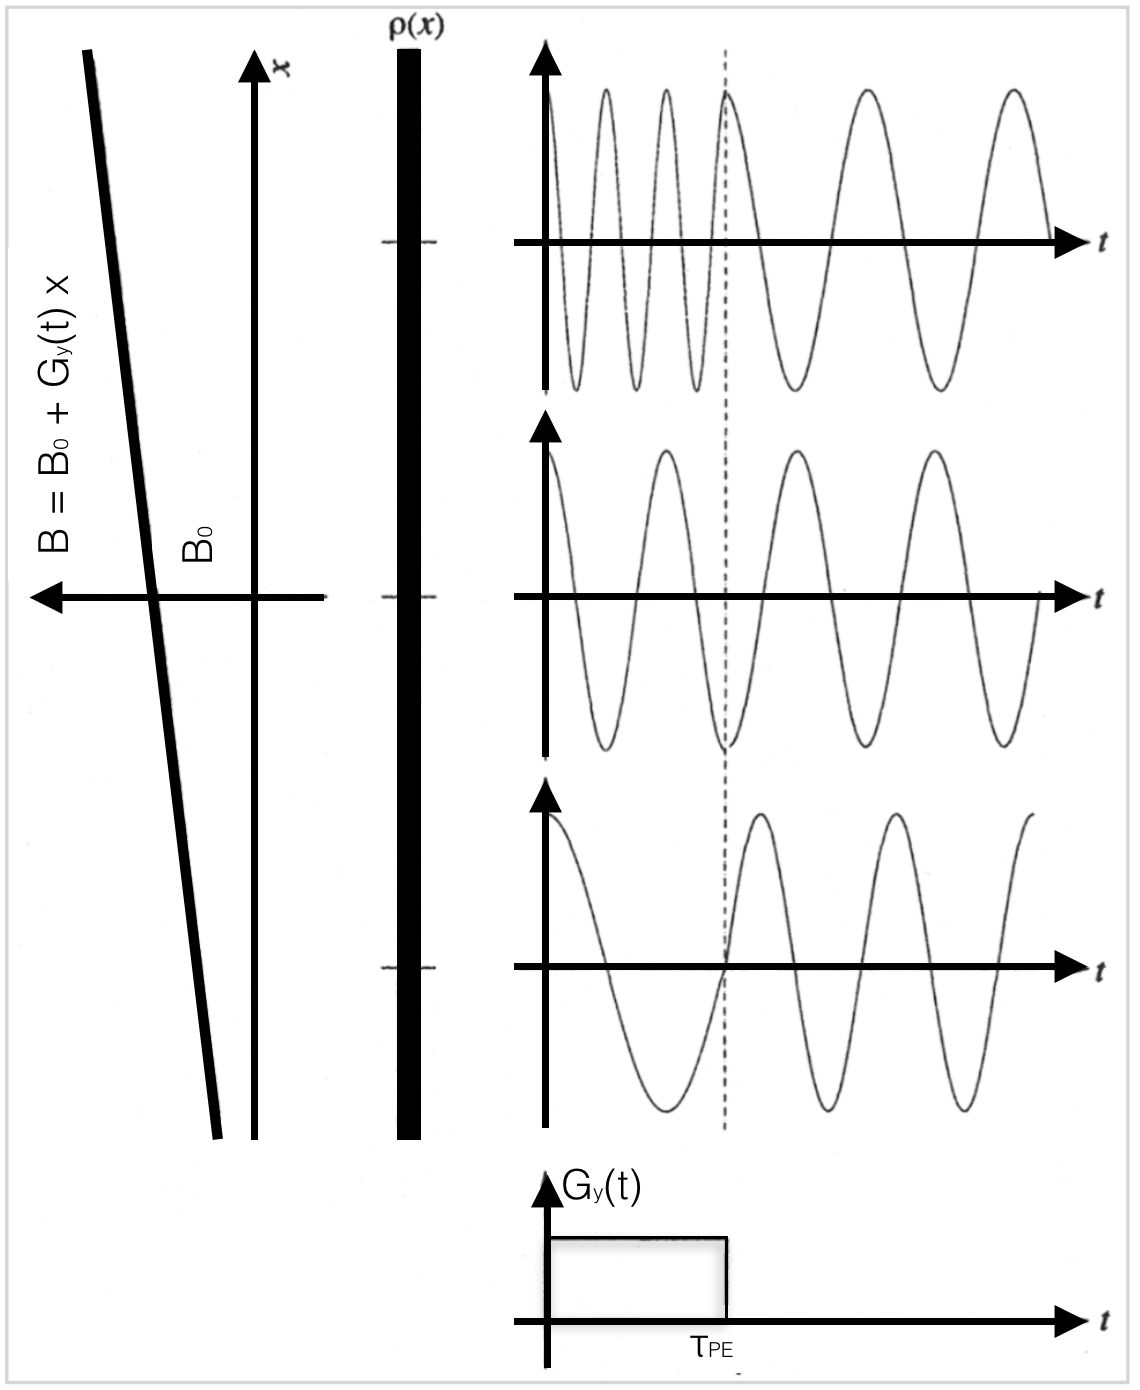
\includegraphics[width=\textwidth]{images/mri/ch10phaseenc}
        \caption{Example of how the phase encoding gradient will affect the signal arising from different locations within a spin system.}
        \label{fig:ch10phaseenc}
    \end{subfigure}
    
    \caption{Frequency encoding and phase encoding are used to spatially localise the signal coming from the sample (Figures adapted from \cite{Liang2000}).}
    \label{fig:ch10freqphaseenc}
\end{figure}

\hfill

% % % % 
\textbf{K-space Representation}
The combination of two perpendicular gradients, one that performs frequency encoding and one that performs phase encoding, leads to the 2D spatial localisation of the slice.
By choosing the slice selection gradient to be in the z-direction, 
only x- and y- gradients are now needed to encode the spatial information in the selected slice.
This information is present in the spatial frequency of the overall detected signal:
\begin{equation}\label{eq:915}
    S(t) = \int \int 
            e^{-t/T_2^*} \rho(x,y) 
                e^{ -i \gamma \int_0^t G_x(t')x + G_y(t')y dt'} dx dy
\end{equation}

By introducing the notion of \textit{spatial frequency} $k = k(t)$ such that:
\begin{equation}\label{eq:kspace}
    k_x(t) = \frac{\gamma}{2 \pi} \int_0^t \vec{G}_x(t') dt' 
    \qquad\text{and}\qquad
    k_y(t) = \frac{\gamma}{2 \pi} \int_0^t \vec{G}_y(t') dt' 
\end{equation}
equation \ref{eq:915} can be rewritten as:
\begin{equation}\label{eq:102}
    S(k_x, k_y) = \int \int e^{-t/T_2^*} \rho(x,y) e^{-i 2 \pi (k_x x + k_y y)} dx dy
\end{equation}

Without taking the relaxation term into account, equation \ref{eq:102} is fundamental to MRI as it is the inverse Fourier transform of the spin density $\rho(x,y)$:
\begin{equation}\label{eq:104}
    \rho(x,y) = \int \int S(k_x,k_y) e^{i 2 \pi (k_x x + k_y y)} dk_x dk_y
\end{equation}

In 2D Cartesian MRI, the signal is collected and stored in a matrix called \textit{k-space} where the axis are the $k_x$ and $k_y$ spatial frequencies. A visual representation of simple 2D Cartesian k-space can be seen in Figure~\ref{fig:ch10kspace}.

\begin{figure}[ht]
    \centering
    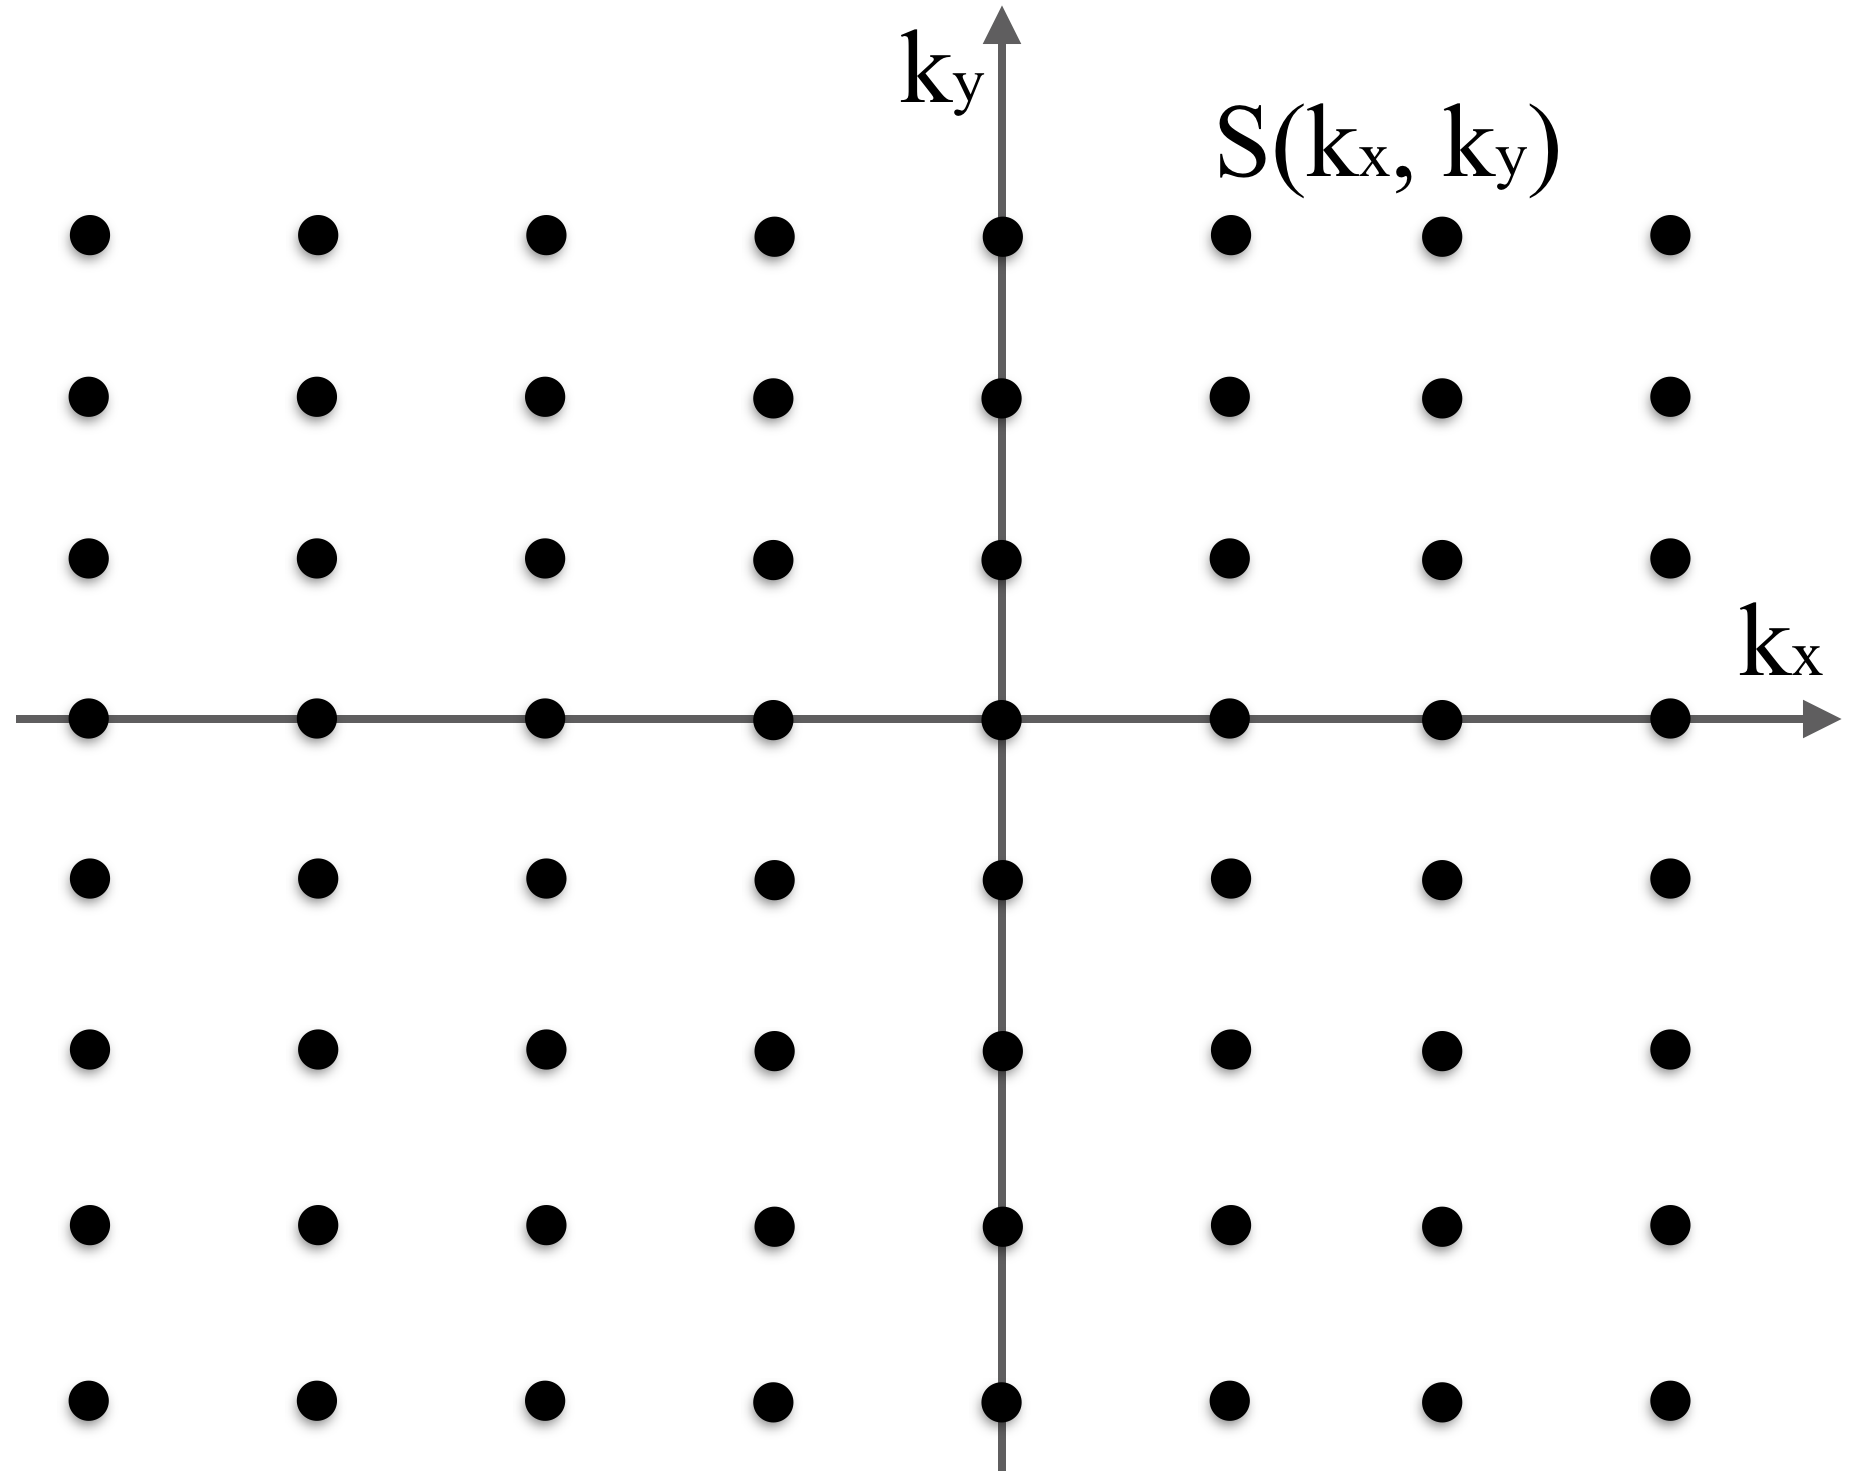
\includegraphics[width=0.5\textwidth,keepaspectratio]{images/mri/ch10kspace}
    \caption{Example of an 8x8 Cartesian k-space. The sampling is asymmetric because it needs to capture the $(k_x, k_y) = (0,0)$ spatial frequencies while keeping an even number of samples in every direction. It is preferred that the number of samples is a power of 2, as the reconstruction method is, in general, a Fast Fourier Transform which works best for those cases.}
    \label{fig:ch10kspace}
\end{figure}

\hfill

% % % % % % % % % % % % 
% % % % % % % % % % % % 
\subsection{Echo Formation}

The signal measured in MRI is called an \textit{echo}. 
Echoes form when a dephased collection of spins is refocused by using one or more applied RF pulses or gradients. 
They are important in MRI because they increase the MR signal due to the rephasing of transverse magnetisation.
There are 3 types of echoes and they can all be obtained by different means: 1) by using a refocusing gradient one can obtain a \textit{gradient echo}, 2) by using an $180^o$ refocusing pulse one can obtain a \textit{spin echo}, and 3) by using 3 rf pulses one can obtain \textit{stimulated echoes}.
The last one is, in general, less useful for imaging and most MRI techniques are tuned to remove the occurance of such echoes.

\hfill

\textbf{Gradient echo.} A gradient echo is obtained by inverting the polarity of the gradient which caused the dephasing. 
This type of echo formation cannot recover the loss of magnetisation due to magnetic field inhomogeneities.
As a consequence, the signal collected for this type of echo will therefore be dependent on $T_2^*$. 
An example of a gradient pulse sequence can be seen in Figure~\ref{fig:gradientecho}.

\hfill

\textbf{Spin echo.} Spin echoes are obtained with an $180^o$ RF pulse. 
After an initial $90^o$ excitation pulse, the spins will start to dephase due to spin-spin interactions and inhomogeneities in the main magnetic field.
The application of the second pulse, the $180^o$ refocusing pulse, will reverse the acquired phase.
This leads to the formation of an echo whose amplitude will no longer depend on $T_2^*$, but on $T_2$.
An example of a spin echo pulse sequence of the $90^o - \tau_1 - 180^o - \tau_2 - \text{Spin-Echo}$ (where $\tau_1 = \tau_2 = T_E/2$) can be seen in Figure~\ref{fig:spinecho}.

\begin{figure}[ht]
\centering
\begin{minipage}{.5\textwidth}
  \centering
  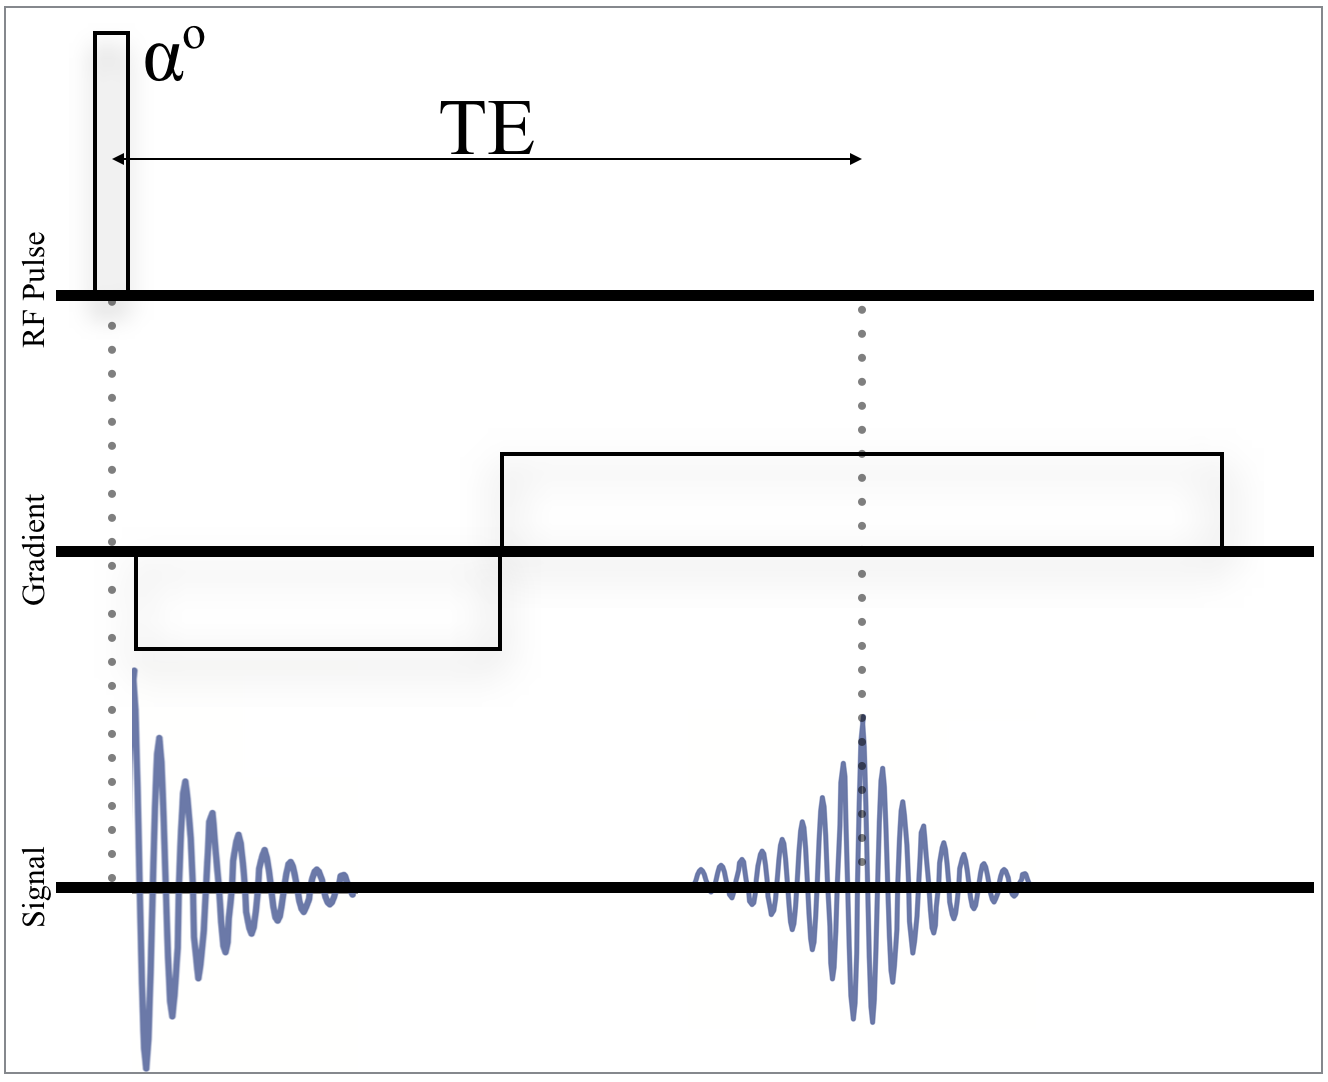
\includegraphics[width=.9\linewidth]{images/mri/gradientecho}
  \captionof{figure}{Example of a gradient echo forming as a result of the application of the second gradient.}
  \label{fig:gradientecho}
\end{minipage}%
\begin{minipage}{.5\textwidth}
  \centering
  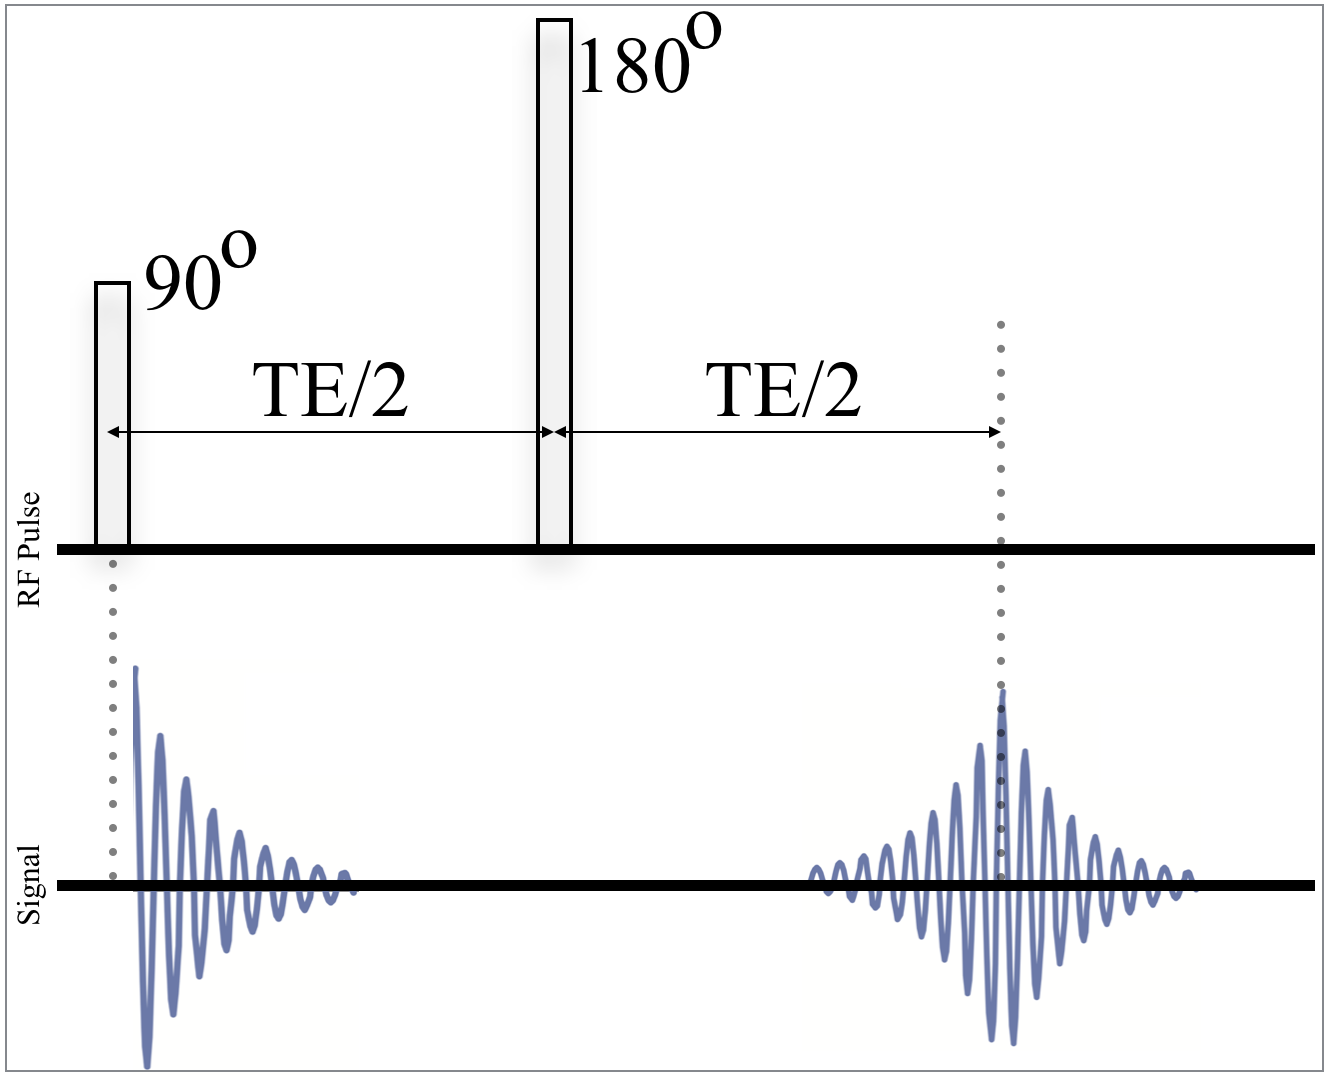
\includegraphics[width=.9\linewidth]{images/mri/spinecho}
  \captionof{figure}{Example of a spin echo forming as a result of the $180^o$ refocusing pulse.}
  \label{fig:spinecho}
\end{minipage}
\end{figure}

\hfill

\textbf{Stimulated echo.} Stimulated echoes are formed after at least 3 RF pulses.
The simplest pulse sequence that gives rise to a stimulated echo is a $90^o - \tau_1 - 90^o - \tau_2 - 90^o - \tau_3 - \text{Stimulated-Echo}$, where $\tau_3 = \tau_1$ is the when the echo forms \cite{Frahm1985}.
Stimulated echoes arise from spins that refocus because of the combination of the three applied RF pulses, together with several other spin echoes \cite{Burstein1996}.
An example of the formation of a stimulated echo is shown in Figure~\ref{fig:stimulatedecho}.

\begin{figure}[ht]
    \centering
    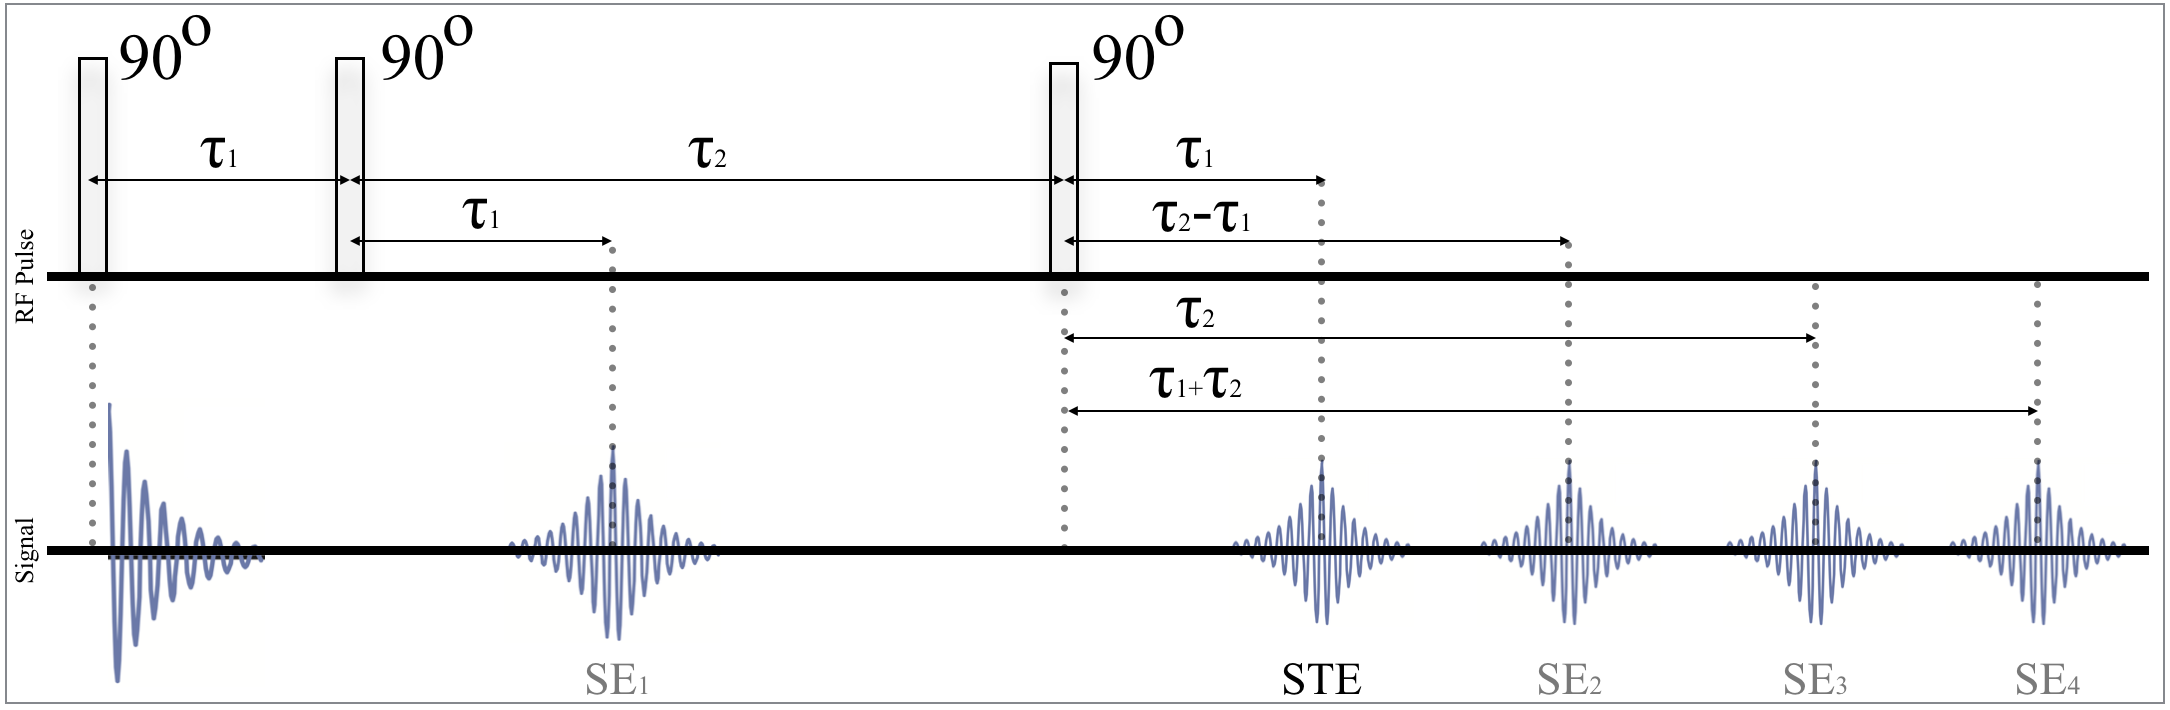
\includegraphics[width=0.95\textwidth,keepaspectratio]{images/mri/stimulatedecho}
    \caption{Example of a stimulated echo forming as a result of 3 $90^o$ RF pulses. The STE forms at $\tau_1$ after the 3rd RF pulse, while the primary SE forms at $\tau_1$ after the 2nd RF pulse. The diagram also shows 3 secondary spin echoes forming after the stimulated echo.}
    \label{fig:stimulatedecho}
\end{figure}

\hfill

% % % % % % % % % % % % % % % 
% % % % % % % % % % % % % % % 
\subsection{Pulse Sequence}

A pulse sequence is a series of magnetic fields used in conjunction with data acquisition to produce MR images.
Pulse sequences are constructed in such a way that they allow the differentiation of tissues by emphasizing in the acquired signal the contribution of the tissue parameters.
In its simplest form, a pulse sequence starts with a $90^o$ excitation pulse applied together with a slice select gradient, to excite the spins found in a certain desired part of the imaged object.
Second, the slice select gradient is followed by an inverse polarity half-area lobe which refocuses the previously dephased spins.
Next, the phase encoding gradient is applied in an orthogonal direction to the slice select gradient, followed by a frequency encoding gradient which will cover the 3rd orthogonal direction.
The frequency encoding gradient is accompanied by data acquisition.
The signal is then demodulated and stored in the spatial frequency matrix called \textit{k-space}.
The final step is then to Fourier transform this matrix and obtain the MR image.

\hfill

% % % % 
\textbf{K-space traversal in 2D Cartesian MRI.}
The pulse sequence used also dictates the way the \textit{k-space} is being filled.
For example, a gradient-echo pulse sequence will fill the matrix line-by-line.
This process can be seen in Figure~\ref{fig:PulseSeqGE}. 
After the slice select gradient is applied, the negative lobe of the phase encoding gradient is played together with the negative lobe of the frequency encoding gradient (step 1).
Next, the signal is acquired while the second (positive) frequency encoding gradient is on (step 2).
This is repeated for different amplitudes of the phase encoding gradient until the entire k-space matrix is filled.

\begin{figure}[ht]
    \centering
    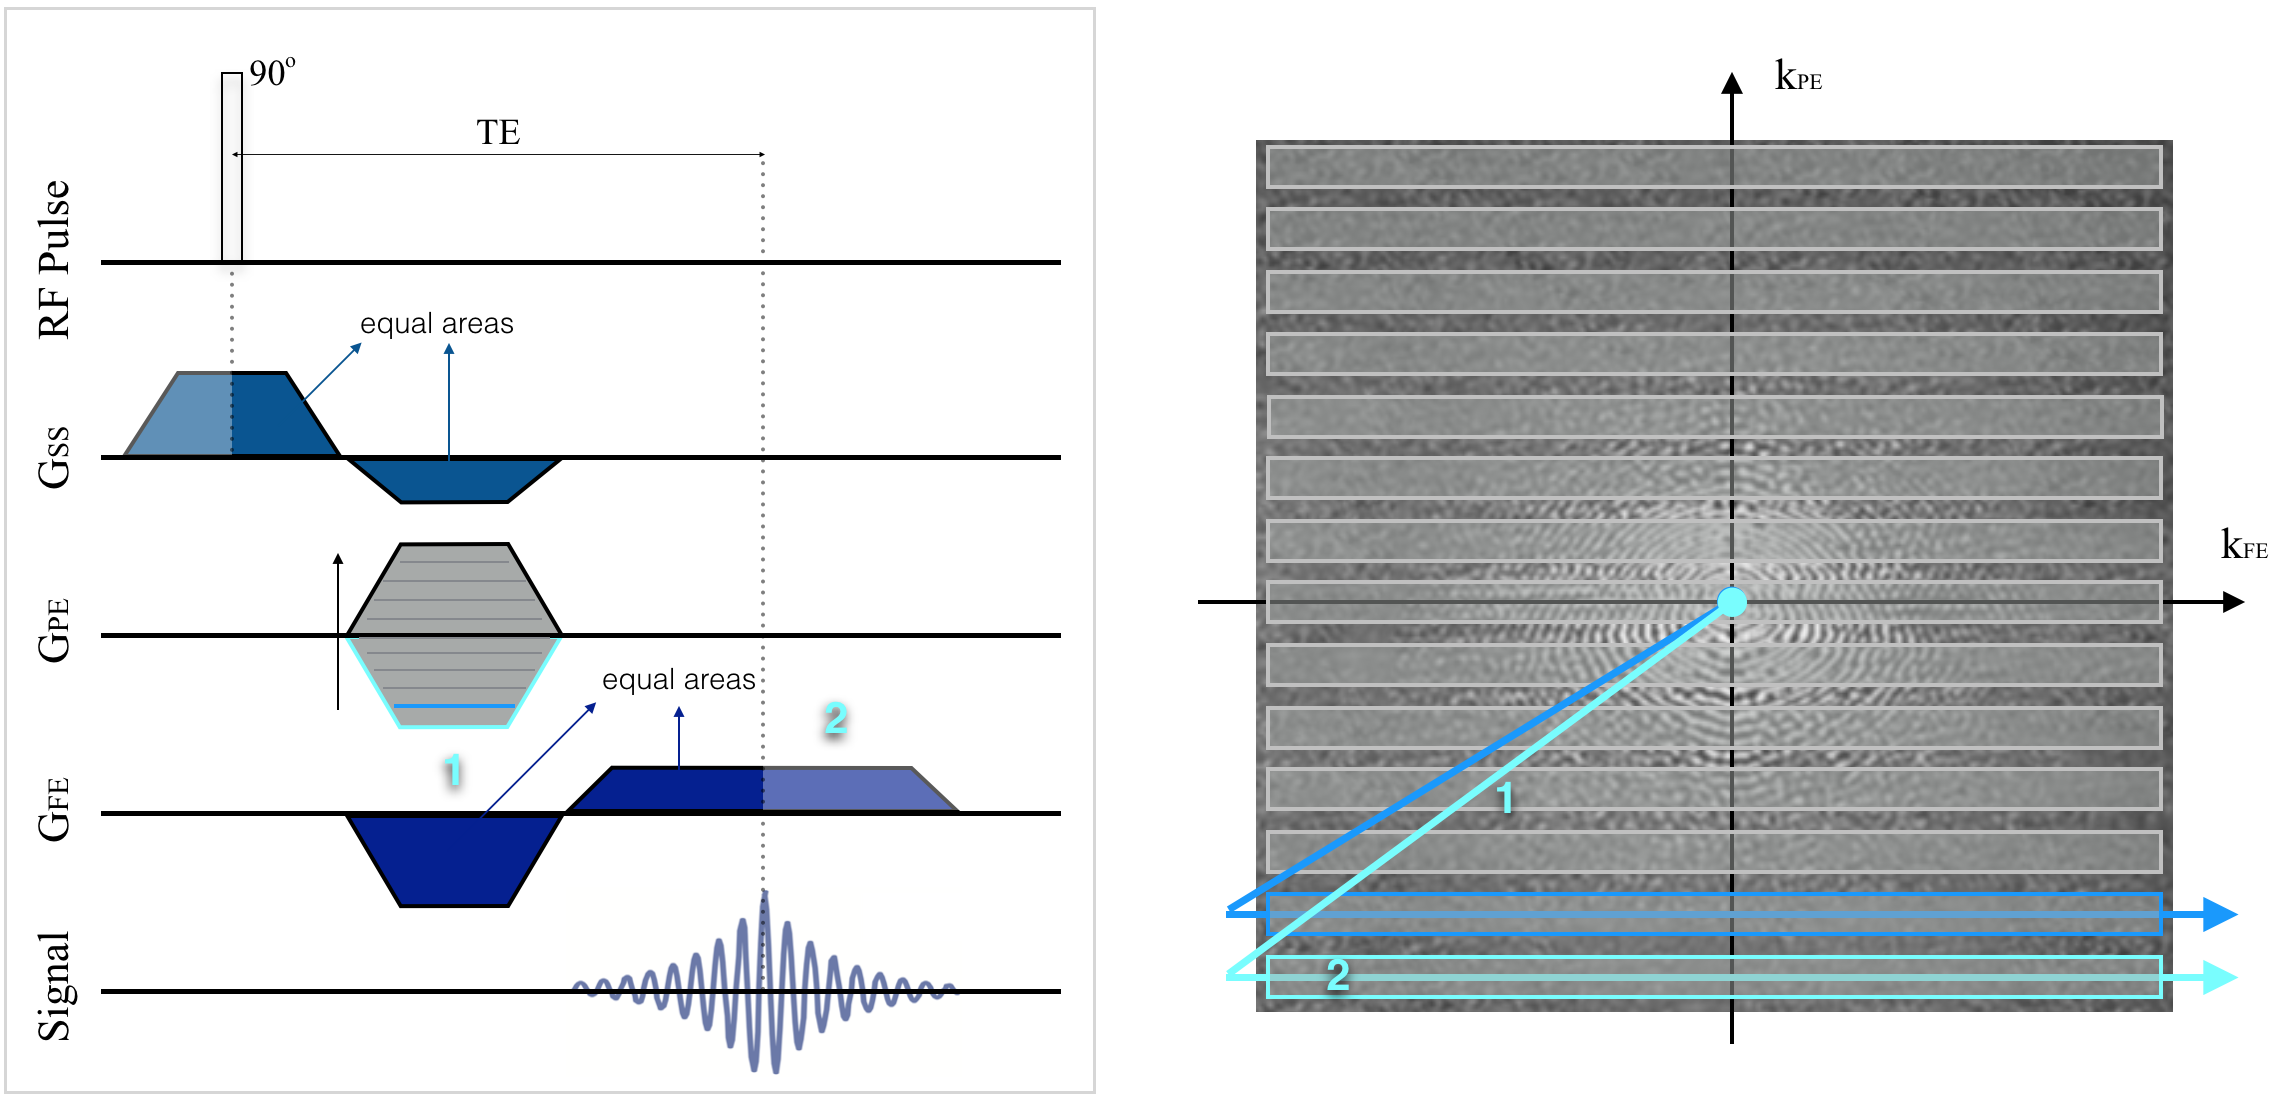
\includegraphics[width=0.95\textwidth,keepaspectratio]{images/mri/PulseSeqGE}
    \caption{Example of a gradient-echo pulse sequence together with the corresponding k-space traversal path.}
    \label{fig:PulseSeqGE}
\end{figure}

The gradient-echo pulse sequence requires a long acquisition time because each line of k-space is acquired separately. 
Echo Planar Imaging (EPI) is a faster method which has been proven to be very useful in a wide variety of MR applications where speed is a requirement.
This method acquires the entire k-space matrix after one excitation pulse (see Figure~\ref{fig:PulseSeqEPI}).
Each line of k-space is traversed either from left to right or from right to left depending on the polarity of the frequency encoding gradient (steps 2 and 4 in the figure).
Moreover, the 'blipped' phase encoding gradients (step 3 in the figure) move the acquisition from one line to the next until the entire matrix is filled.

\begin{figure}[ht]
    \centering
    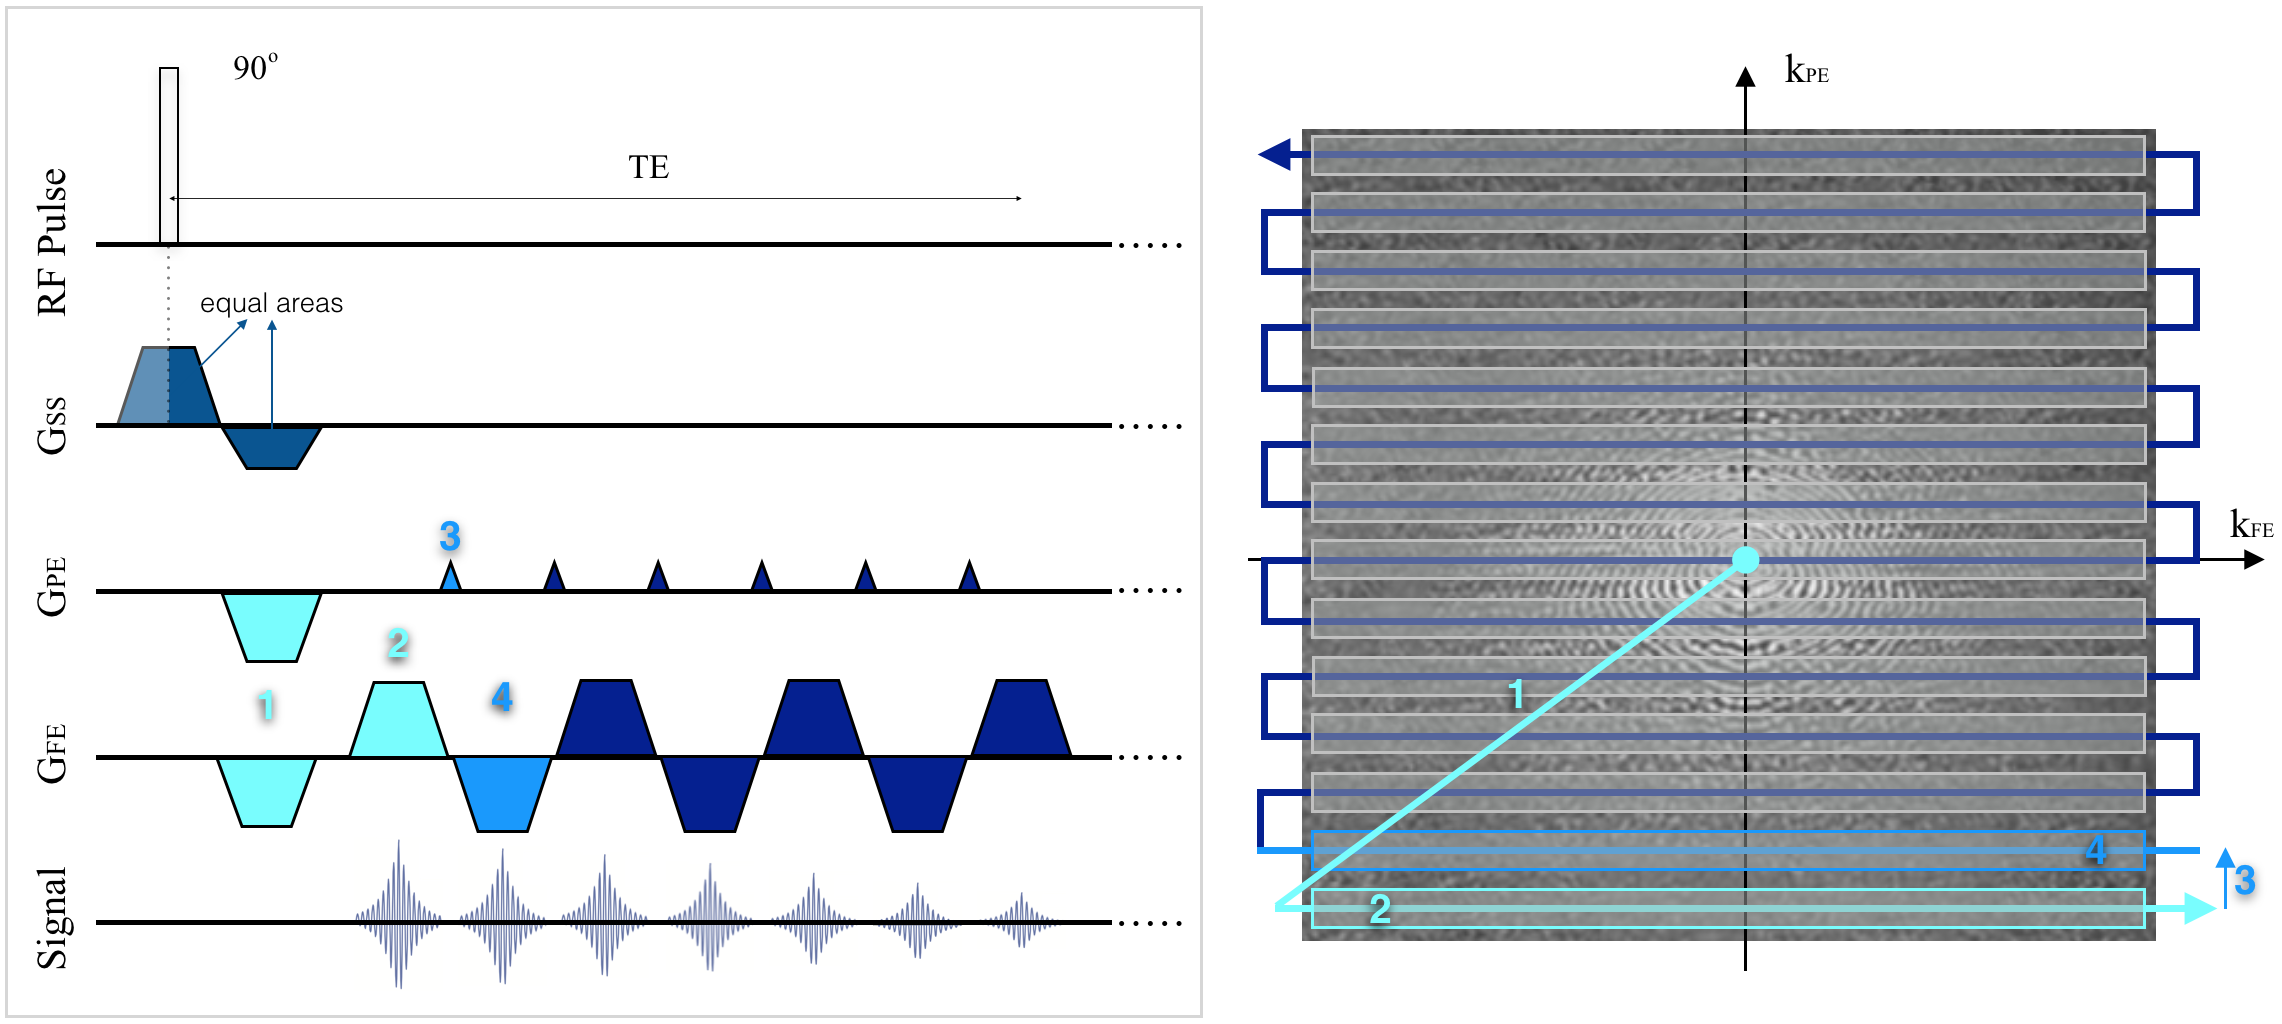
\includegraphics[width=1\textwidth,keepaspectratio]{images/mri/PulseSeqEPI}
    \caption{Example of a gradient-echo EPI pulse sequence together with the corresponding k-space traversal path.}
    \label{fig:PulseSeqEPI}
\end{figure}

\hfill

% % % % % % % % 
\subsection{Image Reconstruction}

The final step of an MRI acquisition protocol is the reconstruction step.
Once all the spatial information data has been collected, a Fast Fourier Transform (FFT) is used to yield an image (Figure~\ref{fig:fourierReconstruction}). 

\hfill

% % % % 
\textbf{Image Resolution.} The relationship between these two Fourier pairs and the properties of the k-space matrix are of utmost importance in MRI because they dictate the quality and resolution of the final image.
The sampling intervals in both frequency encoding and phase encoding directions in k-space are called $\Delta k_x$ and $\Delta k_y$ and are inversely proportional to the image field-of-view (FOV) \cite{Deshmane2012}:
\begin{equation} \label{eq:1210}
    FOV_x = \frac{1}{\Delta k_x} = \frac{1}{\frac{\gamma}{2 \pi} G_x T_s}
\end{equation}
and
\begin{equation} \label{eq:1211}
    FOV_y = \frac{1}{\Delta k_y} = \frac{1}{\frac{\gamma}{2 \pi} \Delta G_y \tau_y}
\end{equation}

From these relationships we can deduce that an increase in sampling frequency leads to a decrease in the FOV $\Delta k_x \uparrow \, \Rightarrow \, FOV_x \downarrow$ and $\Delta k_y \uparrow \, \Rightarrow \, FOV_y \downarrow$.
Moreover, if we multiply the equations above with $1/N_x$ and $1/N_y$ we see that the highest spatial frequencies sampled in k-space $k_{x,max} = \Delta k_x N_x/2 $ and $k_{y,max} = \Delta k_x N_x/2 $ are inversely proportional to the image resolution $\Delta x$ and $\Delta y$.
We can therefore deduce that an increase in $k_{x,max}$ or $k_{y,max}$ leads to an increase in the image resolution: $k_{x,max} \uparrow \, \Rightarrow \, \Delta x \downarrow$ and $k_{y,max} \uparrow \, \Rightarrow \, \Delta y \downarrow$. 
These findings are summarized in the equations below and in Figure~\ref{fig:fourierReconstruction}.

\begin{equation} \label{eq:1212}
    \Delta x = \frac{1}{N_x \Delta k_x} = \frac{1}{2 k_{x,max}} = \frac{1}{\frac{\gamma}{2 \pi} G_x T}
\end{equation}
and
\begin{equation} \label{eq:1213}
    \Delta y = \frac{1}{N_y \Delta k_y} = \frac{1}{2 k_{y,max}} = \frac{1}{\frac{\gamma}{2 \pi} 2 G_{y,max} t_y}
\end{equation}

\begin{figure}[ht]
    \centering
    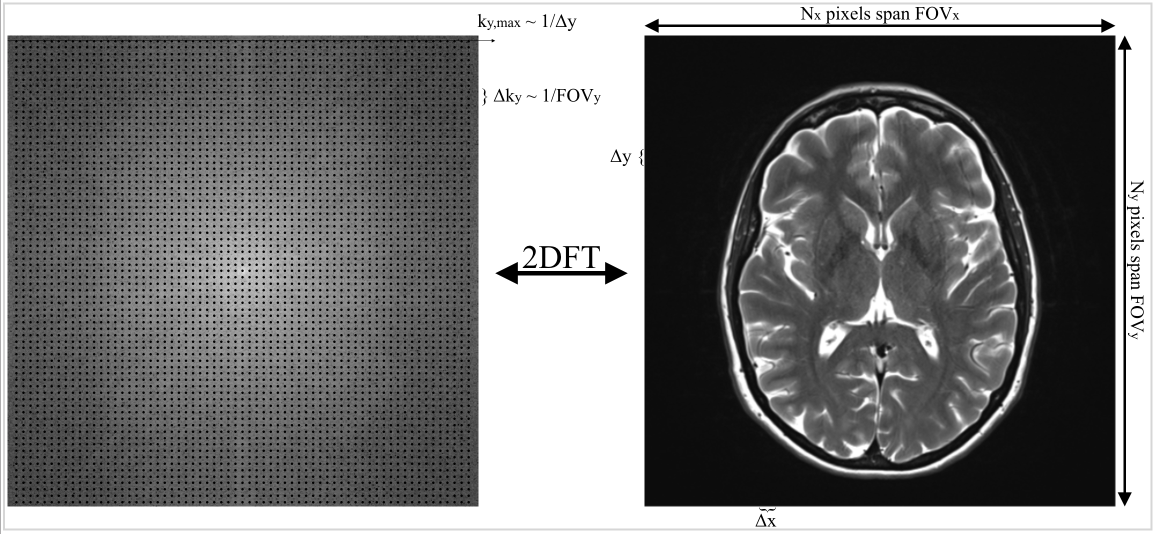
\includegraphics[width=1\textwidth,keepaspectratio]{images/mri/fourierReconstruction}
    \caption{The k-space data and the MR image are Fourier pairs. A 2D Fast Fourier Transform applied on the k-space matrix yields the final image. Properties of the sampling and image resolution are presented briefly.}
    \label{fig:fourierReconstruction}
\end{figure}


\hfill

% % % % 
\textbf{Aliasing.} However, if the sampling rate is not high enough such that the \textit{Nyquist-Shannon} theorem is broken, the final image will suffer from aliasing Artifacts \cite{Deshmane2012}. 
Figure~\ref{fig:fourierReconstructionPartial} shows what happens when undersampling occurs in the phase-encoding direction.

\begin{figure}[ht]
    \centering
    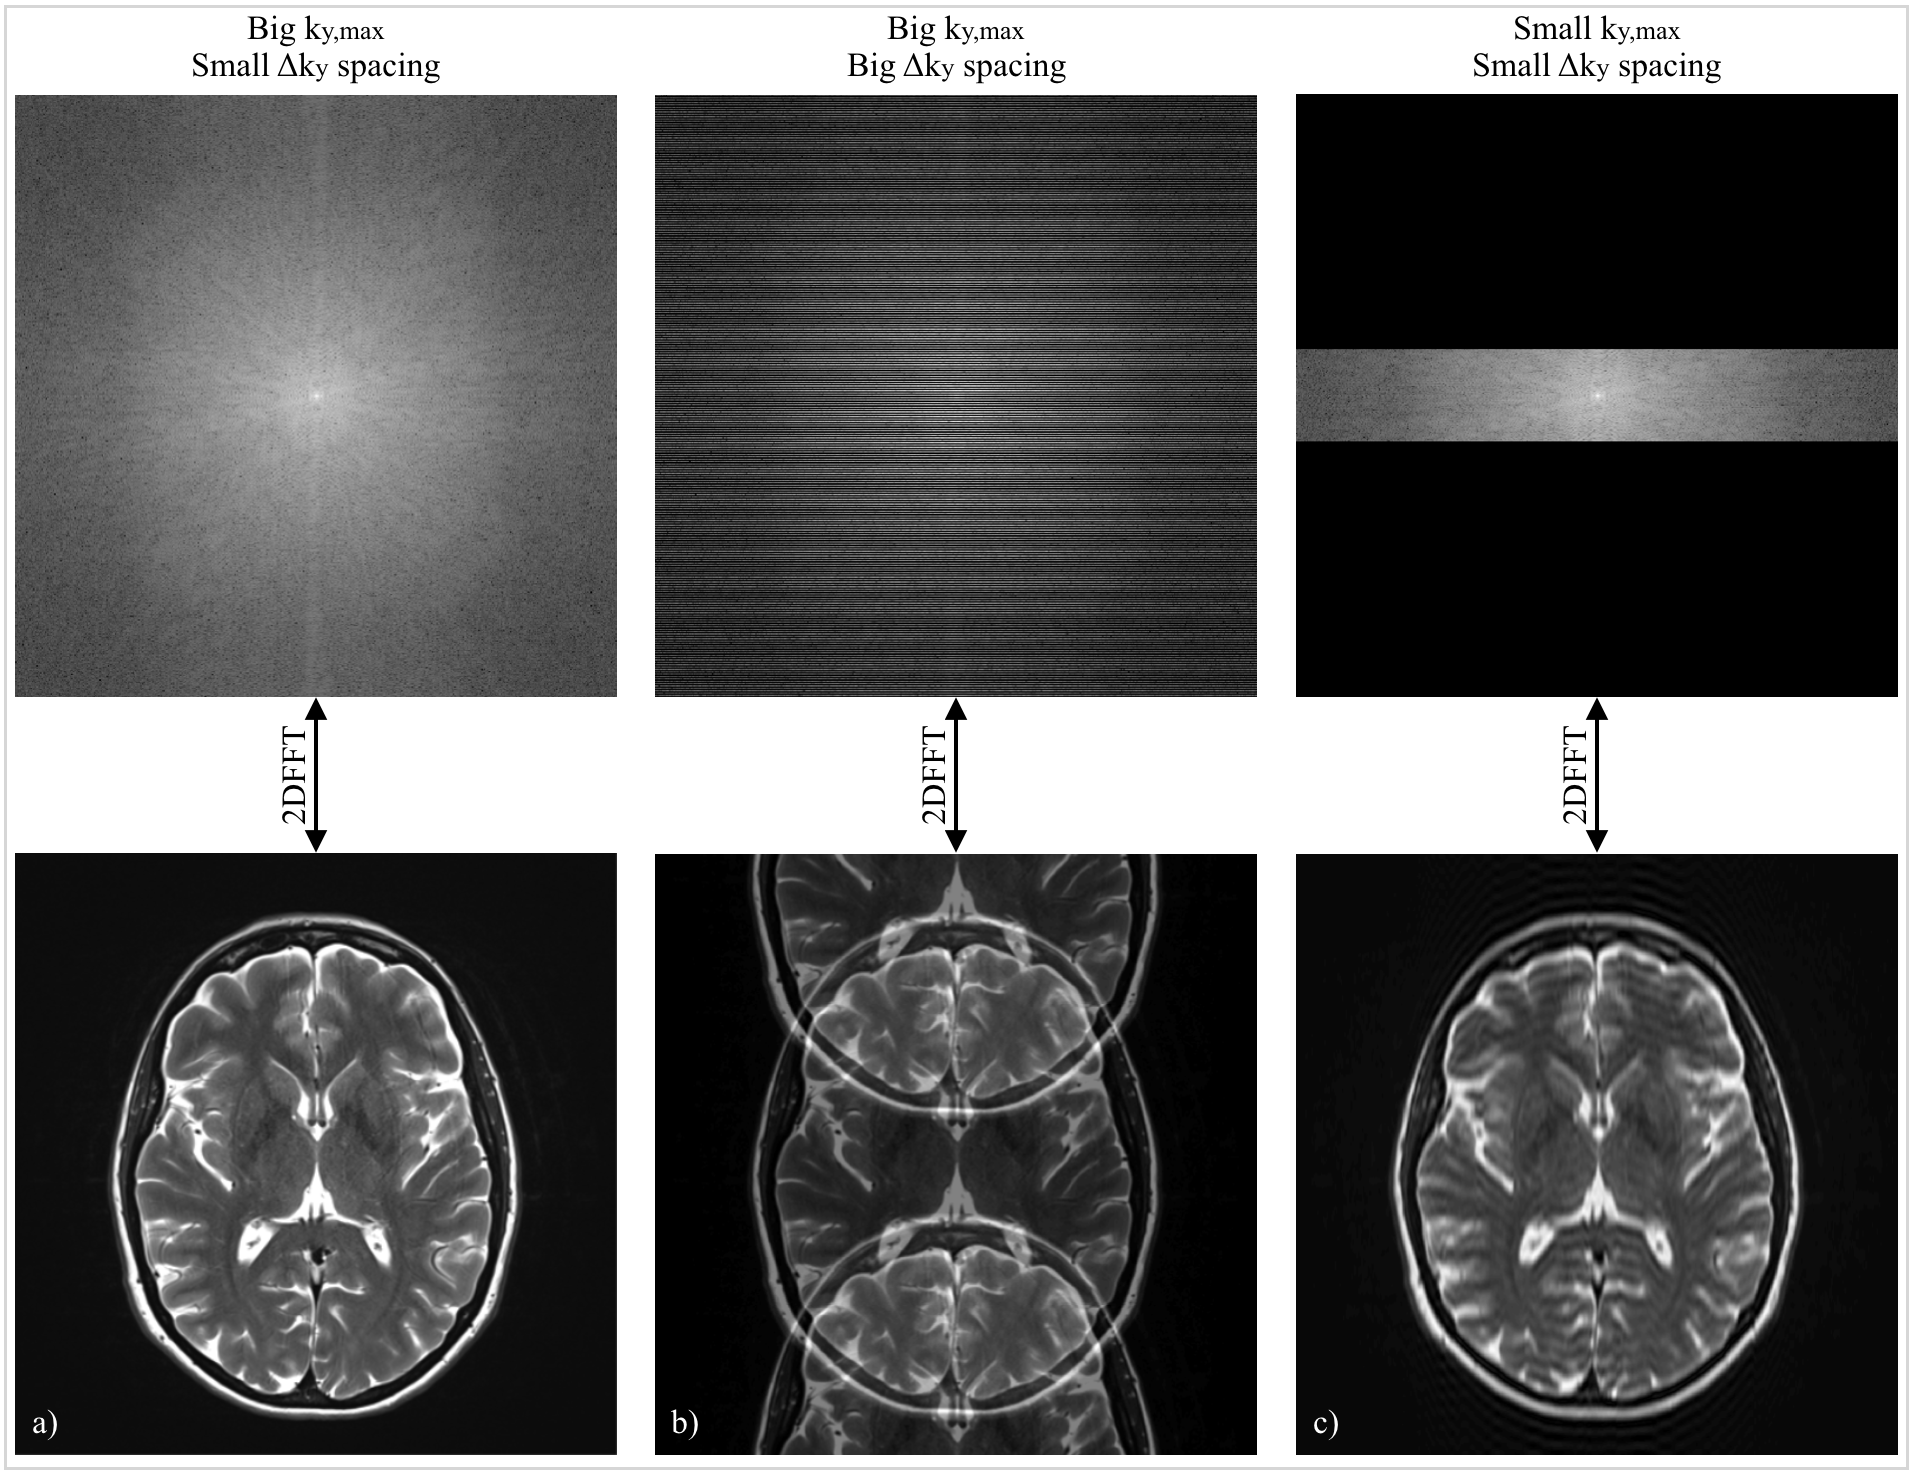
\includegraphics[width=1\textwidth,keepaspectratio]{images/mri/fourierReconstructionPartial}
    \caption{Example of different sampling schemes: a) a fully sampled k-space and the final image, b) an acquisition scheme where every other line of k-space in the phase encoding direction has been skipped; this results in aliasing in the same direction, c) only the low spatial frequencies are kept which results in a blurred image}
    \label{fig:fourierReconstructionPartial}
\end{figure}

\hfill

% % % % % % % % % % % % 
% % % % % % % % % % % % 
\subsection{Image Artifacts}

Image artifacts are defined as false features in the final reconstructed image \cite{Haacke1999}. 
They appear as a consequence of the interaction between the imaging protocol and the object under investigation, as well as from the reconstruction process. 
MR image artifacts come in two flavours, each of which can be further categorised depending on the underlying cause:

\clearpage

\textbf{Technique-related artifacts}
    \begin{itemize}
        \item \textit{Aliasing} is a frequently encountered MRI artifact. 
        As presented before (see Figure~\ref{fig:fourierReconstructionPartial} b)), aliasing can occur in any direction where the signal has not been sampled densely enough to be reconstructed with high fidelity.
        More specifically, aliasing happens as a consequence of the \textit{analog-to-digital} conversion step, where the otherwise continuous signal is being digitized (sampled).
        The signal digitization is equivalent to the multiplication with a `comb' function which, when Fourier transformed, leads to the periodicity of the object.
        Aliasing can be corrected by increasing the sampling rate in the direction where the artifact occurred, or by using more advanced reconstruction methods such as parallel imaging.
        
        \item \textit{Gibbs Ringing} also appear as a consequence of the \textit{analog-to-digital} conversion step.
        However, unlike aliasing where the problem arises due to digitization, ringing results from windowing the data.
        This signal `truncation' directly translates into sampling the data at a finite number of frequencies.
        This results in an oscillating undershoot and overshoot close to step discontinuities.
        In the final images this appears as multiple parallel lines near interfaces with high-contrast.
        
    \end{itemize}

\hfill

\textbf{Tissue-related artifacts}
    \begin{itemize}
        \item \textit{Chemical Shift} refers to the change in resonant frequency of spins due to the interaction with their local molecular environment.
        For example, fat protons experience a slightly lower magnetic field than a neighbouring water proton because they are shielded by their own electron cloud.
        The difference in frequencies is very small, but increases with higher fields magnets ($215$Hz at $1.5$T and $430$Hz at $3$T).
        As a consequence, when both fat and water protons are found in the same voxel during the frequency-encoding part of the sequence, fat protons will be spatially mapped towards the weaker side of the gradient due to their lower precessing frequency.
        This will cause the appearance of a \textit{shift} along the FE direction in the final image. 
        
        \item \textit{Susceptibility} artifacts refer to a wide variety of MR artifacts that are caused by local magnetic field inhomogeneities.
        In MRI, they are generally encountered near metal implants or at air-tissue and air-bone interfaces where the otherwise homogeneous external magnetic field is locally altered.
        There are three ways the final image is affected:
        \begin{enumerate}
            \item Tissue can be mismapped to a different slice due to being incorrectly excited.
            \item Changes in the tissue frequency can cause geometric distortions.
            \item Signal loss can occur due to accelerated transverse relaxation.
        \end{enumerate}
        
        \item \textit{Motion} is ubiquitous in MRI because
        the time required for the majority of MR sequences to collect the necessary data is much longer than most types of physiological motion, including respiratory motion, vessel pulsation, CSF flow and even involuntary patient motion.
        At best, bulk motion can lead to slice misalignment which can be corrected for with registration algorithms.
        However, if motion happens during the acquisition part of the experiment, it can lead to blurring of object edges, ghosting, loss of information or undesired strong signals \cite{Zaitsev2015}.
        It is therefore important to understand how different types of motion affect the final image in order to correct for the unwanted artifacts, either with motion-correction algorithms, or with better imaging techniques.
        
    \end{itemize}

\hfill 

% % % % % % % % % % % % % % % % 
\section{Fast Imaging Using Non-Cartesian K-space Trajectories}\label{chapterlabel2sec13}

The length of an MRI scan is generally longer compared to other medical imaging modalities such as computer tomography.
It is therefore important to achieve high imaging speeds in MRI in order to make it more clinically feasible \cite{Cohen1991}.
However, imaging speed is limited by the physical constraints of the scanner, such as the amplitude and slew rate of the gradients, and by the physiological constraints of the tissue, such as specific absorption rate (SAR) or peripheral nerve stimulation (PNS).

\hfill

One way to reduce scan time is to acquire less k-space data.
Unfortunately, as we have seen before, this leads to aliasing artifacts in the final images \cite{Pusey1988}.
Despite this, the MR literature presents methods to mitigate these artifacts while maintaining the quality of the final images.
Some of these methods exploit the information provided by the receiver coils and fall under the umbrella of parallel imaging techniques \cite{Griswold2002} \cite{Pruessmann2001} \cite{Pruessmann1999} \cite{Seiberlich2008}, 
others exploit the spatial or temporal redundancy of the k-space data \cite{Tsao2012} \cite{Jung2009} \cite{Tsao2003},
while others benefit from the advent of Compressed Sensing in the signal processing world by exploiting sparsity in the transform domain \cite{Lustig2007} \cite{Pedersen2009} or by using incoherent sampling techniques \cite{Candes2006} \cite{Haldar2011}.

\hfill

% % % % % % % % % % % % 
% % % % % % % % % % % % 
\subsection{Non-Cartesian trajectories}

Other fast imaging techniques include the use of non-Cartesian trajectories.
Based on the properties of the trajectories, these sampling schemes can have many advantages over the conventional Cartesian techniques.
One advantage is that these trajectories can be designed to efficiently use the MR gradient hardware in such a way that it leads to a more rapid coverage of k-space \cite{Wright2014}.

\begin{figure}[ht]
    \centering
    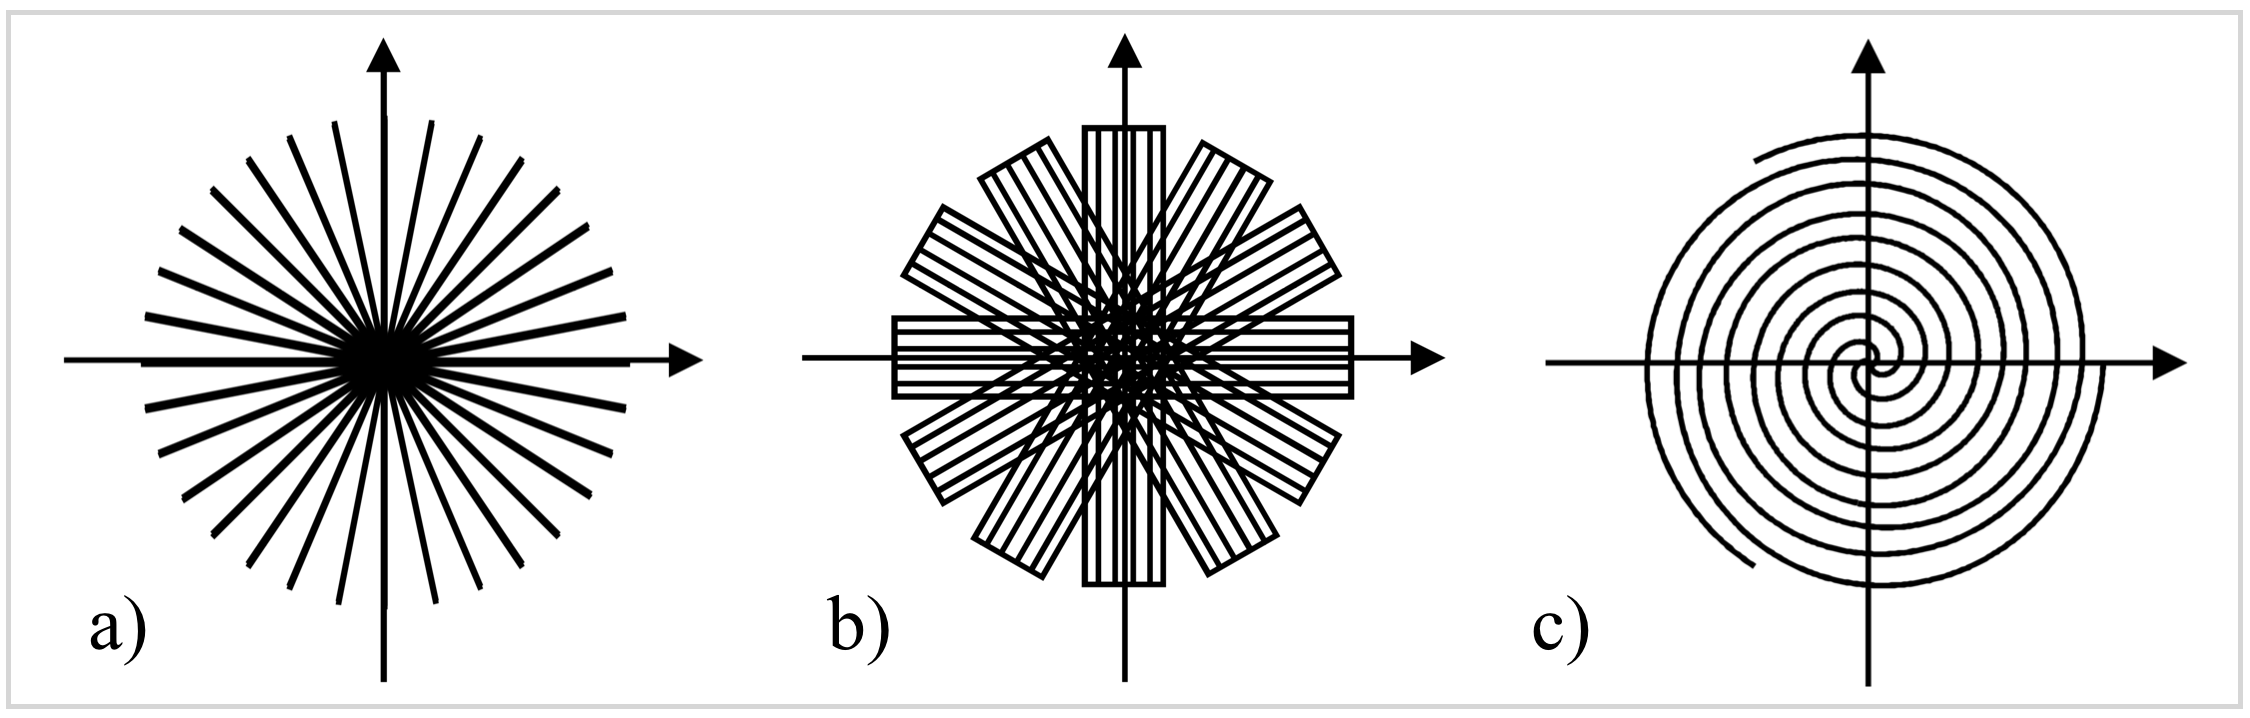
\includegraphics[width=1\textwidth,keepaspectratio]{images/mri/noncarttraj}
    \caption{Example of three different non-Cartesian sampling techniques: a) radial trajectory, b) PROPELLER trajectory and c) spiral trajectory}
    \label{fig:noncarttraj}
\end{figure}

Although there are many non-Cartesian trajectories in the literature, the most popular ones can be seen in Figure~\ref{fig:noncarttraj}.
\textbf{Radial trajectories} (Figure~\ref{fig:noncarttraj} a) are commonly used in 
real-time cardiac imaging because they have the advantage of achieving high temporal resolution by using short echo times \cite{Seiberlich2011} \cite{Schaeffter2001}.
Moreover, due to the inherent oversampling of the center of k-space, radial techniques are known to be more robust to motion or flow artifacts \cite{Pauly1992}.
The \textbf{PROPELER} (Periodically Rotated Overlapping ParallEL Lines with Enhanced Reconstruction) trajectory (Figure~\ref{fig:noncarttraj} b) combines Cartesian and radial sampling in one scheme by simultaneously acquiring a few parallel spokes called `blades'. 
Due to the overlapping central parts, PROPELLER trajectories are commonly used for motion correction \cite{Pipe1999}.
Finally, another common non-Cartesian sampling technique involves \textbf{spiral trajectories} (Figure~\ref{fig:noncarttraj} c). 
These techniques offer a high flexibility in design as spiral trajectories can be constructed to sample k-space either with a constant density pattern \cite{Ahn1986} \cite{Meyer1992} or a variable density pattern \cite{Tsai2000}.
Spiral trajectories are used to reduce motion artifacts in cine cardiac imaging \cite{Kressler2007} and to improve temporal resolution in perfusion imaging \cite{Lee2003}.

\hfill

% % % % % % % % % % % % 
% % % % % % % % % % % % 
\subsection{Gridding}
\label{MRIgridding}

Unlike evenly spaced, uniformly sampled Cartesian k-space data, non-Cartesian trajectories require more complicated algorithms than a simple FFT.
A direct extension of the discrete Fourier Transform for nonrectiliniar data is too computationally slow and therefore impractical.
The alternative is to resample the data onto a Cartesian grid and then apply the FFT.
There are several approaches to this, but the most commonly used one is called `gridding'.

\begin{figure}[ht]
    \centering
    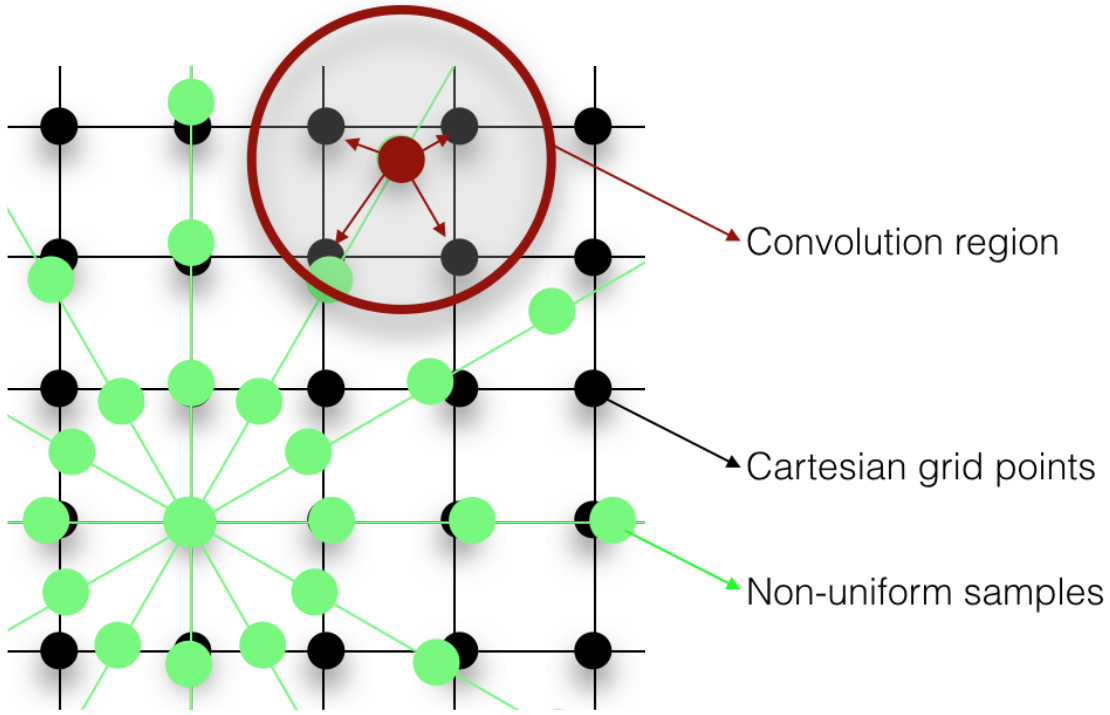
\includegraphics[width=0.7\textwidth,keepaspectratio]{images/mri/gridding}
    \caption{The non-uniformly sampled k-space data points (shown in green) are interpolated onto a Cartesian grid (shown in black). Each sample is convolved with a dedicated kernel (shown in red) and the result is resampled onto the appropriate Cartesian k-space locations.}
    \label{fig:gridding}
\end{figure}

Gridding is a convolution-based reconstruction method that has become popular in MR imaging because it gives good quality results while being faster than most other methods.
This technique relies on estimating a uniformly sampled Cartesian k-space from a non-rectiliniar one (see Figure~\ref{fig:gridding}).
The gridding algorithm is made up of a few steps.
First, if the k-space data has been measured at variable density, each value in the dataset $\big( S(k_i) \big)$ is multiplied with a density correction function $\big( DCF(k_i) \big)$ before interpolation.
Second, each corrected data point ($S'(k_i)$) is convolved with a dedicated kernel $\big( C(k)$ gridding kernel$\big)$ and then resampled onto a Cartesian grid $\big( \Sh (k_j)\big)$. 
These two steps are summarised in the following equations:

\begin{equation}\label{eq:gridding1}
        S'(k_i) = S(k_i) DCF(k_i)
\end{equation}
\begin{equation}\label{eq:gridding2}
        S''(k_j) = [S'(k_i) * C(k)] \Sh (k_j)
\end{equation}

To yield an image, an inverse Fourier transform is applied to the now uniformly sampled k-space data $\big( S''(k_j)\big)$. The convolution with the gridding kernel will lead to a multiplication by the inverse Fourier transform of the kernel $\big( c(\rho_j)\big)$:
\begin{equation}\label{eq:gridding3}
        I''(\rho_j) = \mathcal{F}^{-1} \{ S''(k_j) \} = I(\rho_j) c(\rho_j) \text{ where } c(\rho) = \mathcal{F}^{-1} \{ C(k) \}
\end{equation}

It is therefore important to choose an appropriate kernel function that will not alter the final image.
O'Sullivan found that the best gridding kernel to use would be an infinite sinc function because its transform is rectangular and band-limited \cite{OSullivan1985}.
However, this is not computationally feasible and a compact support function is used instead. 
A finite kernel leads to intensity variation in the image and requires a post-processing step.
This step is called `deapodization' and it involves dividing the reconstructed image by the inverse Fourier transform of the kernel:
\begin{equation}\label{eq:gridding4}
        I(\rho_j) = I''(\rho_j) / c(\rho_j)
\end{equation}

The choice of convolution function is not straightforward.
Jackson et al. \cite{Jackson1991} have conducted a comparative study regarding different filter functions used as gridding kernels.
The conclusion they have reached shows that the Kaiser-Bessel function performs best as the final image is closest to the ideal 'sinc' interpolation.
The Kaiser-Bessel window is therefore the most commonly used kernel in gridding reconstructions.

% % % % % % % % % % % % % % % % 
\section{Fast Imaging Using Steady State Sequences}\label{chapterlabel2sec14}

One other popular way to reduce scan time is to use short repetition times ($T_R$).
$T_R$ is the time from the application of one RF pulse to the application of the next one.
In conventional MRI, repetition times are long enough to allow for full recovery of the longitudinal magnetisation (generally $\geq 5 T_1$) such that at the beginning of the next $T_R$ period the system starts from equilibrium.

\hfill

In 1958, Carr et al \cite{Carr1958} observed that when a spin system is repeatedly excited by a train of equally spaced RF pulses the signal will eventually reach a steady-state.
As the repetition times become shorter, such that they are smaller than the longitudinal relaxation times of the system ($T_R \leq T_1$), the steady-state signal will depend on $T_1$ and $T_R$.
If scan time needs to be reduced even further such that $T_R \leq T_2$, both longitudinal and transverse relaxation are incomplete by the end of the $T_R$ block and the steady-state signal becomes a complicated function of many factors \cite{Hargreaves2012}.

\hfill

Steady-state sequences come in three different flavours, depending on how the residual magnetisation is treated after the imaging portion of the sequence.
These types can be summarised as follows:
\begin{enumerate}
    \item \textit{Steady-state sequences that recover the transverse magnetisation} use balanced gradients, i.e. all the gradients have zero zeroth moment over each repetition time.
    
    \item \textit{Steady-state sequences which average out the transverse magnetisation across a voxel} use `spoiler' gradients at the end of each $T_R$ block.
    
    \item \textit{Steady-state sequences that eliminate the transverse magnetisation} use `spoiler' gradients and vary the phase of each RF pulse.
\end{enumerate}

In the following sections the focus will be on further reviewing two of the most widely used steady-state sequences, the balanced steady-state free precession sequence (bSSFP) and the fast imaging with steady state precession sequence (FISP).

\hfill

% % % % % % % % % % % % 
% % % % % % % % % % % % 
\subsection{bSSFP}
\label{MRIBSSFP}

The balanced steady-state free precession sequence recovers the transverse magnetisation at the end of each $T_R$ period by using balanced (fully rewound) gradients in all directions.
An example of such a sequence can be seen in Figure~\ref{fig:bssfp}.

\begin{figure}[ht]
    \centering
    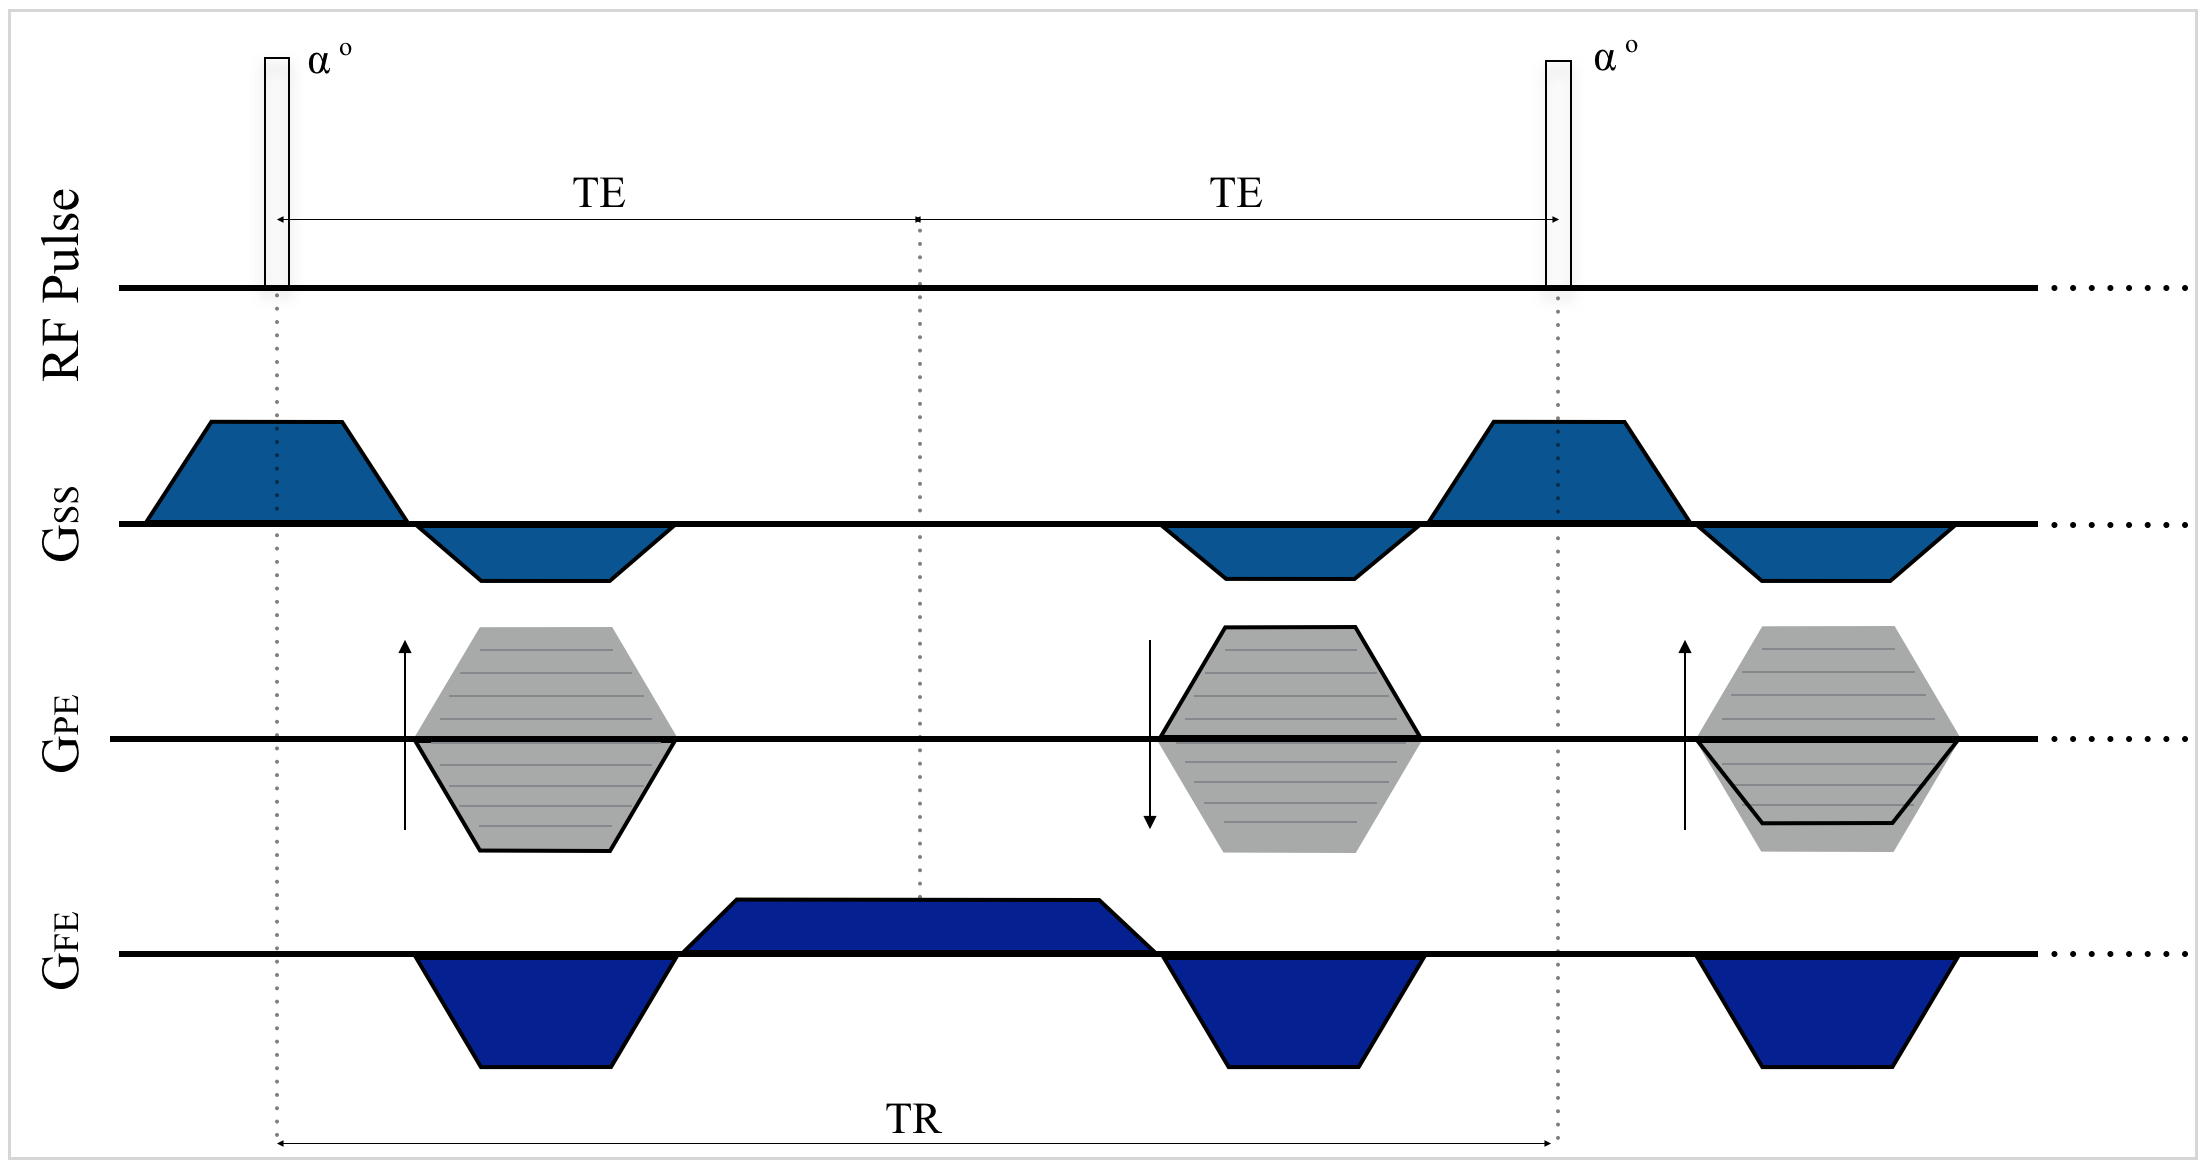
\includegraphics[width=1\textwidth,keepaspectratio]{images/mri/bssfp2}
    \caption{Example of a balanced steady state free precession sequence (bSSFP). 
    In this type of sequence all gradients on all directions have a net moment of zero at the end of each repetition period.}
    \label{fig:bssfp}
\end{figure}

To better understand the magnetisation dynamics in a sequence with constant $T_R$ and repeated RF pulses of flip angle $\alpha$ and phase angle $\phi = 0$, let us first define a spin ensemble with equilibrium magnetisation $M_0$ and with relaxation constants $T_1$ and $T_2$.
At any time $t$ during the sequence, the magnetisation vector can be described as $M(t) \equiv (M_x(t), M_y(t), M_z(t))$.
In between two consecutive RF pulses the magnetisation vector will relax.
Moreover, if there are any spatially invariant static field inhomogeneities $\Delta B$ present,
the phase of the spins will change over a given repetition time period.
This phase will be determined by $\beta(t) = \Delta \omega t = \gamma \Delta B t$, which becomes $\beta(T_R) = \gamma \, \Delta B \, T_R$ at the end of the repetition time.
By defining the magnetisation vector prior to the $n^{th}$ RF pulse as: $M^-(n) \equiv (M_x^-(n), M_y^-(n), M_z^-(n))$ and the magnetisation vector immediately after the $n^{th}$ RF pulse as: $M^+(n) \equiv (M_x^+(n), M_y^+(n), M_z^+(n))$, we are now in a position to describe the dynamics of the total magnetisation in this sequence.

\hfill

At the end of the $n^{th}$ repetition period, immediately before the $(n+1)^{th}$ RF pulse, the magnetisation vector can be written as:
\begin{equation}\label{eq:ssfp}
    M^-(n+1) = R_z(\beta) D(T_R) R_x(\alpha) M^-(n) + C(T_R)
\end{equation}
where the rotation matrices $R_z$ and $R_x$ and the relaxation matrices $D$ and $C$ have been previously described.

\hfill

When the system reaches steady-state the magnetisation vectors can be set to: $M^-(n+1) = M^-(n)$ and $M^+(n) = M^+(n-1)$. 
As $n$ approaches $\infty$, the solutions to equation \ref{eq:ssfp} are (the details of which can be found in \cite{Haacke1999} and \cite{Dharmakumar2005}):
\begin{equation}
    \begin{split}
        M_x^- (\infty) &= M_0 (1-E_1) \frac{E_2 \, sin \alpha  \, sin \beta}{d} \\
        M_y^- (\infty) &= M_0 (1-E_1) \frac{E_2  \, sin \alpha \,  (cos \beta - E_2)}{d} \\
        M_z^- (\infty) &= M_0 (1-E_1) \frac{[(1 - E_2  \, cos \beta) - E_2  \, cos \alpha  \, (cos \beta - E_2)]}{d} 
    \end{split}
\end{equation}
and
\begin{equation}
    \begin{split}
        M_x^+ (\infty) &= M_x^- (\infty) \\
        M_y^+ (\infty) &= M_0 (1-E_1) \frac{sin \alpha  \, (1 - cos \beta  \, E_2)}{d} \\
        M_z^+ (\infty) &= M_0 (1-E_1) \frac{[E_2 (E_2 - cos\beta) + (1-E_2  \, cos\beta)  \, cos \alpha]}{d} 
    \end{split}
\end{equation}
where $E_1 \equiv e^{-T_R/T_1}$, $E_2 \equiv e^{-T_R/T_2}$ and 
$d = (1-E_1 cos \alpha) (1 - E_2 cos\beta) - E_2 (E_1 cos\alpha) (E_2 - cos \beta)$.

\hfill

It is evident from the above equations that the signal in bSSFP is a complicated function of RF flip angle, $T_1$ and $T_2$ relaxation times and the resonance offset angle.
From the dependence on the $\beta$ angle we can also conclude that inhomogeneities in the main magnetic field will change the signal.
Indeed, different off-resonance angles affect the signal differently and this is summarised in Figure~\ref{fig:sssignal} for two different RF pulse angles.

\begin{figure}[ht]
    \centering
    \begin{subfigure}[b]{1\textwidth}
        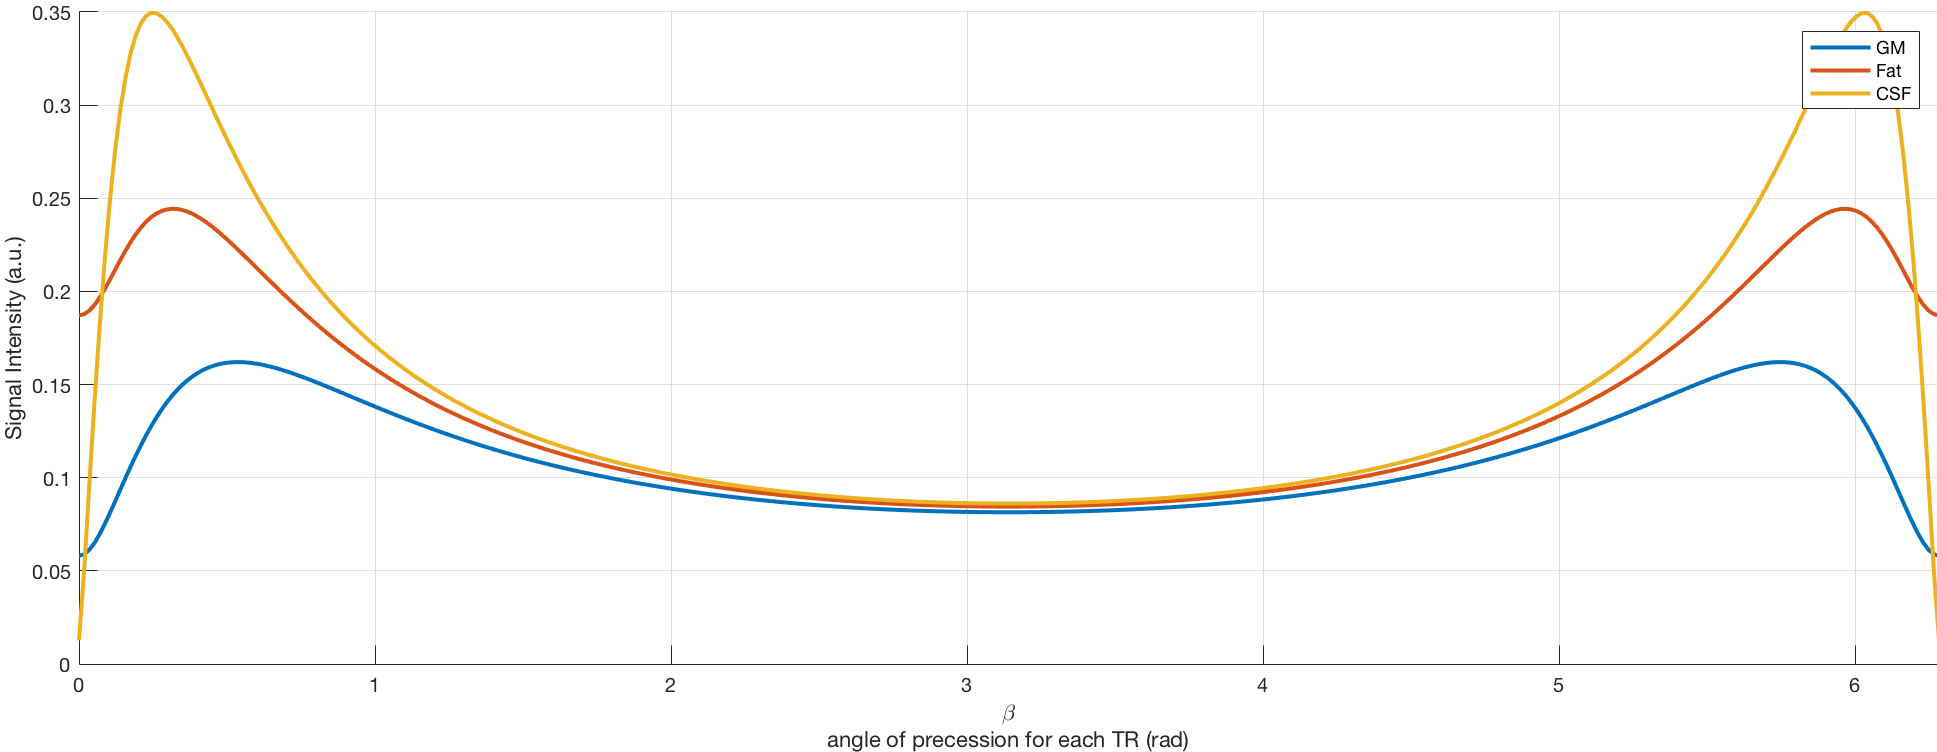
\includegraphics[width=\textwidth]{images/mri/ssFA10}
    \end{subfigure}
    
    \begin{subfigure}[b]{1\textwidth}
        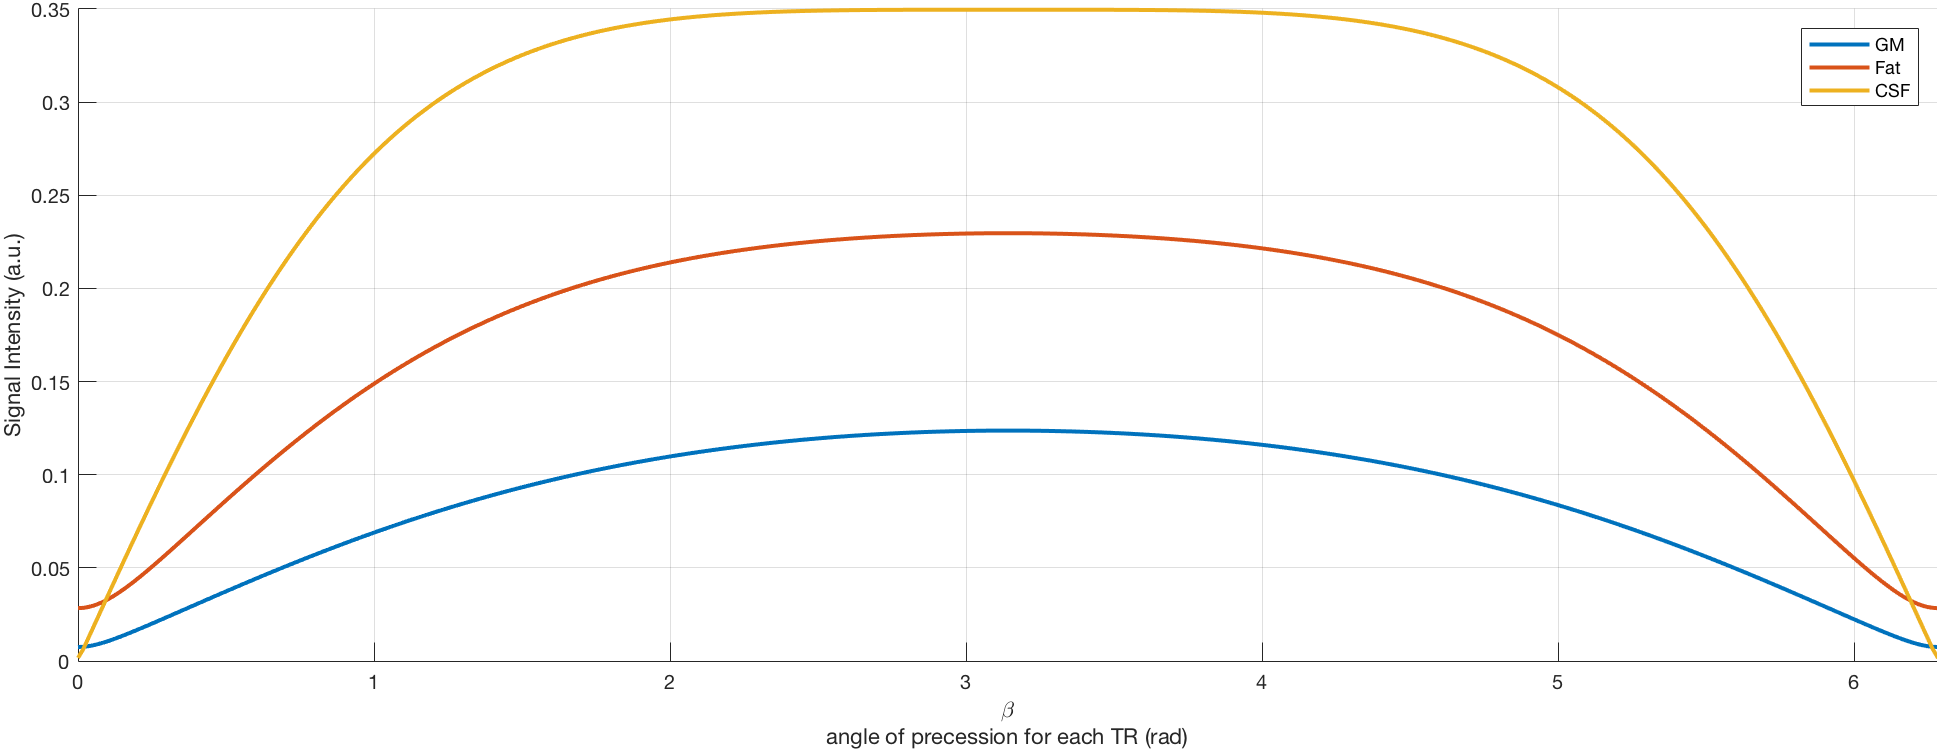
\includegraphics[width=\textwidth]{images/mri/ssFA70}
    \end{subfigure}
    
    \caption{Plot of the magnitude of the signal after reaching steady-state for $T_R = 10ms$ and $T_E = 5ms$ for different tissue types and for a) RF pulse flip angle $\alpha = 10^o$ and b) RF pulse flip angle $\alpha = 70^o$}
    \label{fig:sssignal}
\end{figure}

In spite of its high sensitivity to $B_0$ inhomogeneities which causes `banding artifacts' to appear in the final reconstrcted images, bSSFP-type sequences are used clinically today and are known commercially as: True-FISP, FIESTA, Balanced-FFE or True SSFP \cite{Hargreaves2012}.
These sequences yield the highest signal among all the other rapid gradient-echo sequences and give a contrast of $T_2/T_1$ \cite{Scheffler2003}.
Moreover, bSSFP sequences have been used for quantitative imaging \cite{Schmitt2004b} \cite{Gloor2008} and, more recently, in magnetic resonance fingerpriting \cite{Ma2013}.

\hfill

% % % % % % % % % % % % 
% % % % % % % % % % % % 
\subsection{FISP}
\label{MRIFISP}

A different flavour of a steady-state sequence uses gradient `spoilers' at the end of each $T_R$ block.
This type of sequence is known in the literature as a fast imaging with steady state precession (FISP) sequence.
A typical FISP sequence is shown in Figure~\ref{fig:fisp}.
Unlike bSSFP, the precession of each individual spin during each repetition time is now induced by the spoiler gradients who are strong enough to dominate over inhomogenenties.
In fact, gradient spoilers are constructed in such a way that they achieve an integer number of $\pi$ dephasing across a voxel.
This leads to a slight signal loss because the signal arising from one voxel is now an average over the bSSFP signal.

\begin{figure}[ht]
    \centering
    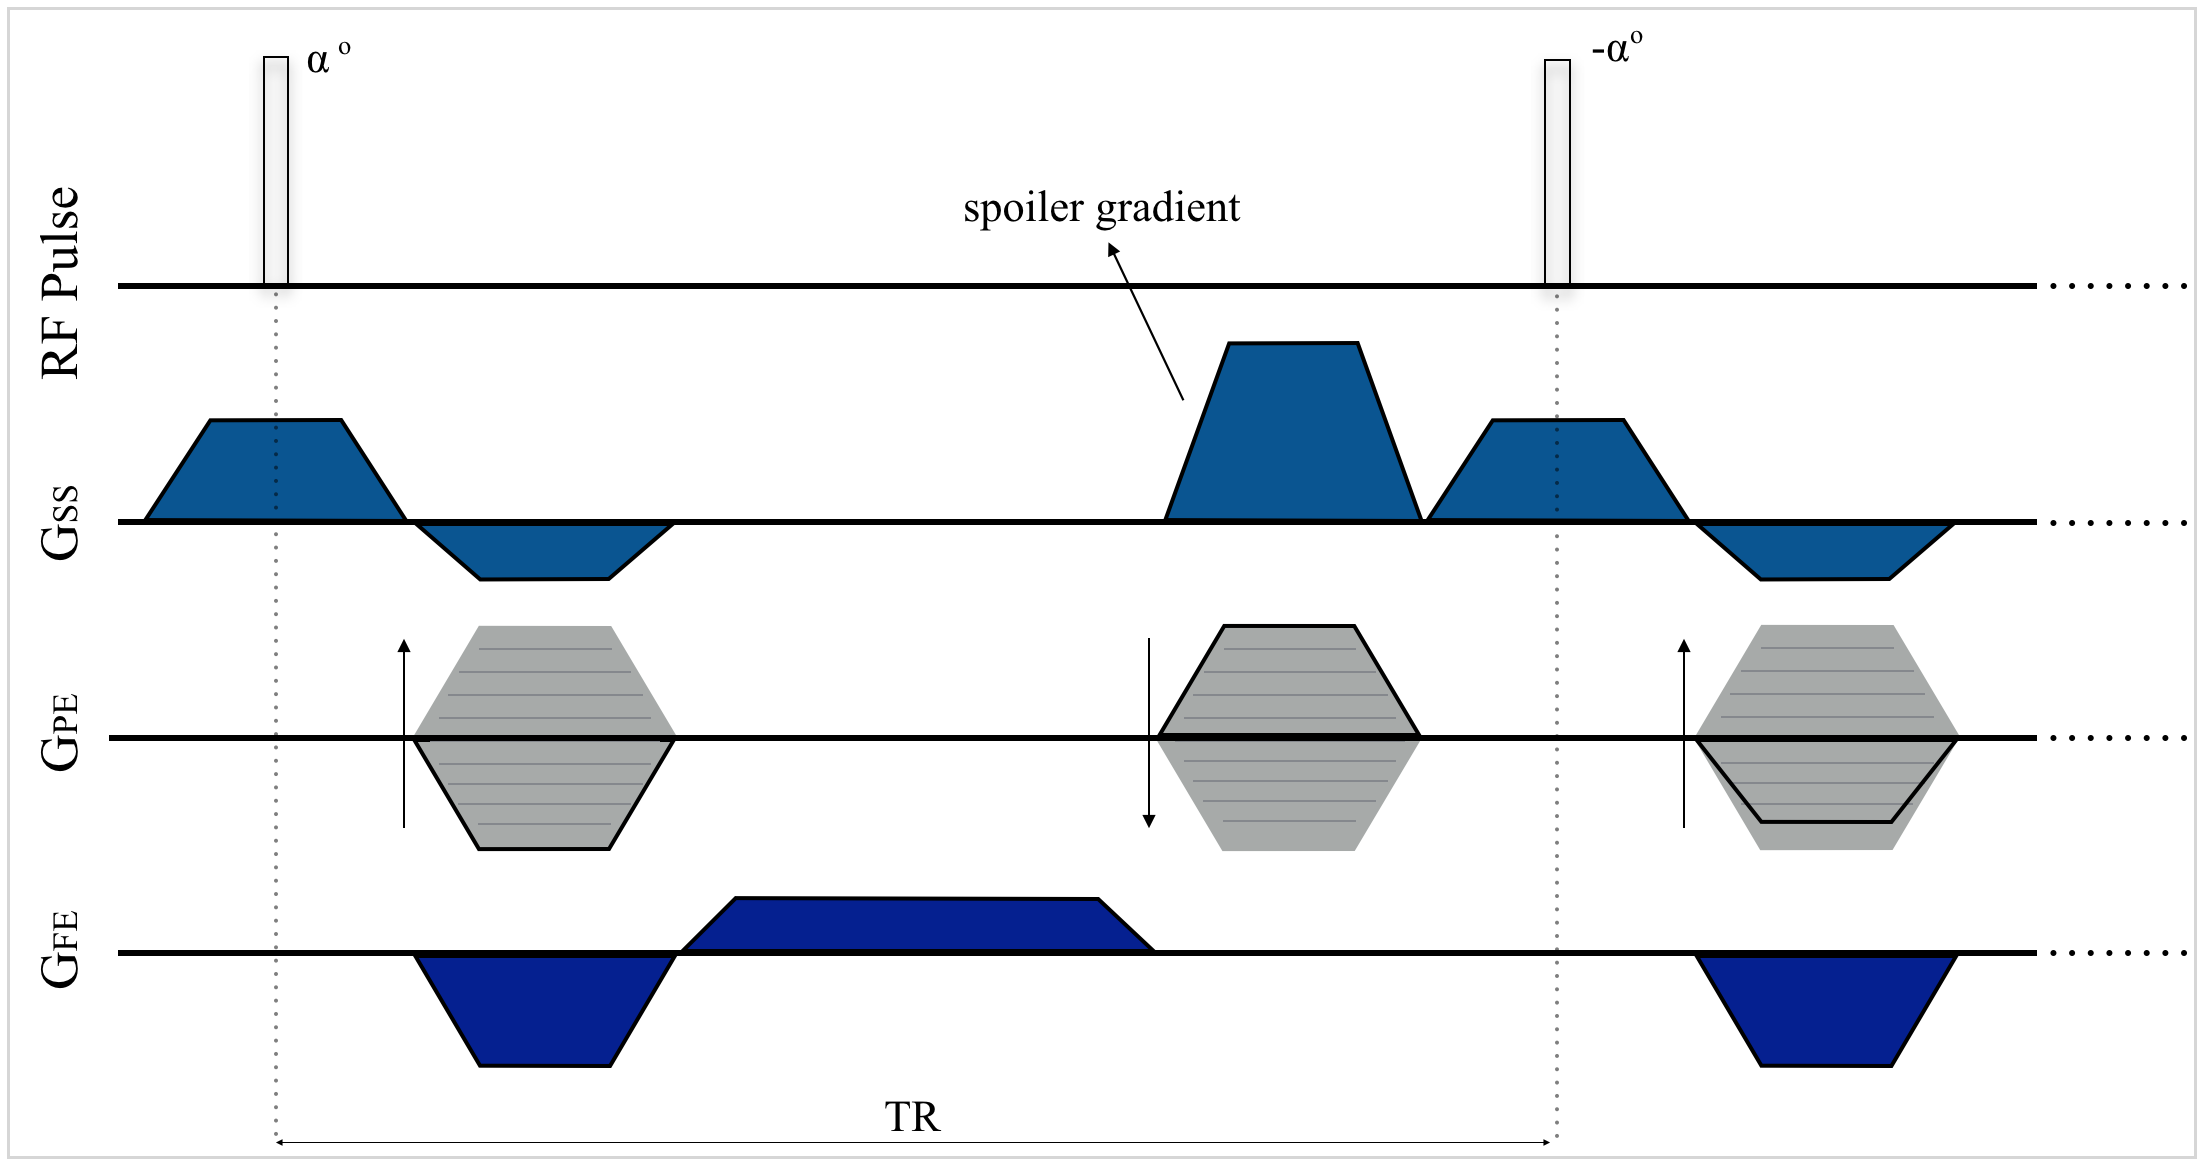
\includegraphics[width=1\textwidth,keepaspectratio]{images/mri/fisp}
    \caption{Example of a fast imaging with steady state precession sequence (FISP). 
    In this type of sequence gradient spoilers are added to one or more axis in each repetition period.}
    \label{fig:fisp}
\end{figure}

The aim of these types of sequences is to avoid the banding artifacts present in bSSFP.
Gradient spoilers can be added to any axis of the sequence or a combination of axis, but it is more common that they are found on the slice selection axis.
While the signal is lower than in bSSFP, it is still a function of $T_2/T_1$ .
Commercially, FISP-type sequences are known as: FE, FFE, GRASS, GRE, FISP, FAST \cite{Hargreaves2012}.
As with bSSFP, the FISP sequence was used by Jiang et al. \cite{Jiang2015} in magnetic resonance fingerprinting to quantify the $T_1$ and $T_2$ relaxation times of the tissue.
